%%%%%%%%%%%%%%%%%%%%%%%%%%%%%%%%%%%%%%%%%
% Journal Article
% LaTeX Template
% Version 1.3 (9/9/13)
%
% This template has been downloaded from:
% http://www.LaTeXTemplates.com
%
% Original author:
% Frits Wenneker (http://www.howtotex.com)
%
% License:
% CC BY-NC-SA 3.0 (http://creativecommons.org/licenses/by-nc-sa/3.0/)
%
%%%%%%%%%%%%%%%%%%%%%%%%%%%%%%%%%%%%%%%%%

%----------------------------------------------------------------------------------------
%	PACKAGES AND OTHER DOCUMENT CONFIGURATIONS
%----------------------------------------------------------------------------------------

\documentclass[twoside]{article}

\usepackage{lipsum} % Package to generate dummy text throughout this template

\usepackage[sc]{mathpazo} % Use the Palatino font
\usepackage[T1]{fontenc} % Use 8-bit encoding that has 256 glyphs
\linespread{1.05} % Line spacing - Palatino needs more space between lines
\usepackage{microtype} % Slightly tweak font spacing for aesthetics

\usepackage[hmarginratio=1:1,top=32mm,columnsep=20pt]{geometry} % Document margins
\usepackage{multicol} % Used for the two-column layout of the document
\usepackage[hang, small,labelfont=bf,up,textfont=it,up]{caption} % Custom captions under/above floats in tables or figures
\usepackage{booktabs} % Horizontal rules in tables
\usepackage{float} % Required for tables and figures in the multi-column environment - they need to be placed in specific locations with the [H] (e.g. \begin{table}[H])
\usepackage{hyperref} % For hyperlinks in the PDF

\usepackage{lettrine} % The lettrine is the first enlarged letter at the beginning of the text
\usepackage{paralist} % Used for the compactitem environment which makes bullet points with less space between them

\usepackage{abstract} % Allows abstract customization
\renewcommand{\abstractnamefont}{\normalfont\bfseries} % Set the "Abstract" text to bold
\renewcommand{\abstracttextfont}{\normalfont\small\itshape} % Set the abstract itself to small italic text

\usepackage{titlesec} % Allows customization of titles
\renewcommand\thesection{\Roman{section}} % Roman numerals for the sections
\renewcommand\thesubsection{\Roman{subsection}} % Roman numerals for subsections
\titleformat{\section}[block]{\large\scshape\centering}{\thesection.}{1em}{} % Change the look of the section titles
\titleformat{\subsection}[block]{\large}{\thesubsection.}{1em}{} % Change the look of the section titles

\usepackage{fancyhdr} % Headers and footers
\pagestyle{fancy} % All pages have headers and footers
\fancyhead{} % Blank out the default header
\fancyfoot{} % Blank out the default footer
\fancyhead[C]{M. Miller and J.W. Baker} % Custom header text
\fancyfoot[RO,LE]{\thepage} % Custom footer text

%---------------------
%extra
\usepackage[comma,square]{natbib}

%% The amssymb package provides various useful mathematical symbols
\usepackage{amssymb}
%% The amsthm package provides extended theorem environments
%% \usepackage{amsthm}

%% The lineno packages adds line numbers. Start line numbering with
%% \begin{linenumbers}, end it with \end{linenumbers}. Or switch it on
%% for the whole article with \linenumbers after \end{frontmatter}.
\usepackage{lineno}

%% natbib.sty is loaded by default. However, natbib options can be
%% provided with \biboptions{...} command. Following options are
%% valid:

%%   round  -  round parentheses are used (default)
%%   square -  square brackets are used   [option]
%%   curly  -  curly braces are used      {option}
%%   angle  -  angle brackets are used    <option>
%%   semicolon  -  multiple citations separated by semi-colon
%%   colon  - same as semicolon, an earlier confusion
%%   comma  -  separated by comma
%%   numbers-  selects numerical citations
%%   super  -  numerical citations as superscripts
%%   sort   -  sorts multiple citations according to order in ref. list
%%   sort&compress   -  like sort, but also compresses numerical citations
%%   compress - compresses without sorting
%%
%% \biboptions{comma,round}

% \biboptions{}

% if you have landscape tables
\usepackage[figuresright]{rotating}

% put your own definitions here:
%   \newcommand{\cZ}{\cal{Z}}
%   \newtheorem{def}{Definition}[section]
%   ...
\usepackage{bbm}

% add words to TeX's hyphenation exception list
%\hyphenation{author another created financial paper re-commend-ed Post-Script}

% declarations for front matter

% use eps figures
\usepackage{epstopdf}
%\usepackage{ecrc}

\newcounter{ead}
\gdef\emailauthor#1#2{\stepcounter{ead}%
     \g@addto@macro\@elseads{\raggedright%
      \let\corref\@gobble
      \eadsep\texttt{#1} (#2)\def\eadsep{\unskip,\space}}%
}


%----------------------------------------------------------------------------------------
%	TITLE SECTION
%----------------------------------------------------------------------------------------

\title{\vspace{-15mm}\fontsize{24pt}{10pt}\selectfont\textbf{Coupling mode-destination accessibility with seismic risk assessment to identify at-risk communities}} % Article title

\author{
 \textsc{Mahalia Miller}\thanks{Corresponding author: Phone: +1-617-692-0574. Department of Civil and Environmental Engineering, Stanford University, 473 Via Ortega, MC 4020, Stanford, CA 94305, United States. Current address: Google, 345 Spear St., Floor 4, San Francisco, CA 94114, United States.}\\
  \texttt{mahalia@alum.mit.edu}
  \and
 \textsc{Jack W. Baker}\thanks{Department of Civil and Environmental Engineering, Stanford University, 473 Via Ortega, MC 4020, Stanford, CA 94305, United States. URL:  web.stanford.edu/~bakerjw/}\\
  \texttt{bakerjw@stanford.edu}
%  \\ 
%  \texttt{Stanford University, 473 Via Ortega, MC 4020, Stanford, CA 94305, United States}
}


% \author{Mahalia Miller}
%%  \ead{mahalia@alum.mit.edu}
%%  \contactphone{+1-617-692-0574}
%% \fntext[label2]{Present address: Google Inc., 345 Spear St., Floor 4, San Francisco, CA 94114, United States}
%% \cortext[cor1]{Corresponding author: Phone: +1-617-692-0574}
%% \fntext[label3]{Current address: Google, 345 Spear St., Floor 4, San Francisco, CA 94114, United States}
%  \author{Jack W. Baker}
% \ead{bakerjw@stanford.edu}
% \ead[url]{web.stanford.edu/~bakerjw/}
% \address{Stanford University, 473 Via Ortega, MC 4020, Stanford, CA 94305, United States}

%\address[label1]{Stanford University, Stanford, CA USA}
%\address[label2]{Stanford University, Stanford, CA USA}

%\address[label1]{Department of Civil and Environmental Engineering, Stanford University, 439 Panama Mall, MC:3037, Stanford, CA 94305, United States\fnref{label3}}


%\author{
%\large
%\textsc{John Smith}\thanks{A thank you or further information}\\[2mm] % Your name
%\normalsize University of California \\ % Your institution
%\normalsize \href{mailto:john@smith.com}{john@smith.com} % Your email address
%\vspace{-5mm}
%}

\date{}

%----------------------------------------------------------------------------------------

\begin{document}

\maketitle % Insert title

\thispagestyle{fancy} % All pages have headers and footers

%----------------------------------------------------------------------------------------
%	ABSTRACT
%----------------------------------------------------------------------------------------

\begin{abstract}
In this paper, we develop a framework for coupling mode-destination accessibility with quantitative seismic risk assessment to identify communities at high risk for travel disruptions after an earthquake. Mode-destination accessibility measures the ability of people to reach destinations they desire%; it is calculated as the log value of the sum of a function of the utilities of each destination over all possible destinations and travel modes, where the utility decreases if getting to that destination is more costly or time-intensive
. We use a probabilistic seismic risk assessment procedure, including a stochastic set of earthquake events, ground-motion intensity maps, damage maps, and realizations of traffic and accessibility impacts. For a case study of the San Francisco Bay Area, we couple our seismic risk framework with a practical activity-based traffic model. As a result, we quantify accessibility risk probabilistically by community and household type. We find that accessibility varies more strongly as a function of travelers' geographic location than as a function of their income class, and we identify particularly at-risk communities.  We also observe that communities more conducive to local trips by foot or bike are predicted to be less impacted by losses in accessibility. This work shows the potential to link quantitative risk assessment methodologies with high-resolution travel models used by transportation planners. Quantitative risk metrics of this type should have great utility for planners working to reduce risk to a region's infrastructure systems.
%In this paper, we develop a framework for coupling mode-destination accessibility with a quantitative seismic-risk assessment to identify communities at a high risk for travel disruptions after an earthquake. For a case study of the San Francisco Bay Area, we find that accessibility varies more strongly from location to location than between income classes, and we identify particularly at-risk communities.  We also observe that communities more conducive to local trips by foot or bike are predicted to be less impacted by losses in accessibility. 

\end{abstract}
\smallskip
\noindent \textbf{Keywords.} Infrastructure, Risk, Earthquakes, Transportation Network, Accessibility

%----------------------------------------------------------------------------------------
%	ARTICLE CONTENTS
%----------------------------------------------------------------------------------------

%\begin{multicols}{1} % Two-column layout throughout the main article text
\linenumbers

%% main text
\section{Introduction}
\label{sec:accIntro}
Seismic risk assessment in earthquake engineering tends to focus on buildings, bridges, and the performance of infrastructure systems. For measuring the performance of transportation systems, researchers typically use engineering-based metrics such as the post-earthquake connectivity loss, which quantifies the decrease in the number of origins or generators connected to a destination node~\cite[e.g.,][]{duenas-osorio_seismic_2007}, or the post-earthquake travel distance between two locations of interest~\cite[e.g.,][]{chang_probabilistic_2000}. These frameworks have provided insight into seismic vulnerability and possible risk mitigation, but do not directly quantify ramifications for people. 

In the field of vulnerability sciences, researchers have long stressed the importance of the impact on human welfare from earthquakes. For example, Bolin and Stanford write that,```Natural' disasters have more to do with the social, political, and economic aspects than they do with the environmental hazards that trigger them. Disasters occur at the interface of vulnerable people and hazardous environments"~\cite{bolin_northridge_1998}. A recent World Bank and United Nations report echoed this idea that the effects on human welfare turn natural hazards into disasters~\cite{the_world_bank_and_the_united_nations_natural_2010}.
Historical events demonstrate the complex social effects of earthquakes. For example, on one hand the 1994 Northridge earthquake caused major damage to nine bridges, which, while significant, represented only 0.5\% of the bridges estimated by Caltrans to have experienced significant shaking~\cite{california._dept._of_transportation._post_earthquake_investigation_team_northridge_1994}. On the other hand, over half of businesses reported closing after the earthquake, with 56\% citing the ``inability of employees to get to work" as a reason~\cite{tierney_business_1997}. Furthermore, the total economic cost of transport-related interruptions (``commuting, inhibited customer access, and shipping and supply disruptions") from this earthquake is estimated at 2.16 billion USD (2014)~\cite{gordon_transport-related_1998}, using the consumer price index to account for inflation.

%  %$1.5 billion, or 27.3%
%of all local business interruption $1.5 billion, or 27.3%
%of all local business interruption
%Additionally, the complex social causes and impacts of this earthquake have been well-studied in the sociology field~\cite{bolin_northridge_1998}.


%~\cite{tierney_foreshadowing_2006}, the author writes that "Disasters result not from physical disaster agents, such as hurricanes, tornados, and earthquakes, but rather from the juxtaposition of three factors: (1) the disaster agent itself--whether a hurricane, earthquake, tornado, or some technological or human-induced event; (2) the physical setting affected by the disaster, including characteristics of the built environment (e.g., structures not built to survive the physical impact of the disaster agent) and environmental features that serve to either mitigate the effects of disasters or make them more severe (e.g., diminished wetlands that could have cushioned the impacts of Katrina); and (3) population vulnerability, a complex construct that includes such factors as; proximity to physical disaster impacts; material resources (income and wealth); race, ethnicity, gender, age; knowledge concerning recommended safety measures; and factors associated with social and cultural capital" and 


Some researchers have measured the impact of earthquakes on transportation infrastructure using the cumulative extra time needed for travel due to damage, sometimes called travel time delay~\cite[e.g.,][]{kiremidjian_seismic_2007,jayaram_efficient_2010}. This performance measure captures basic re-routing due to road closures and identifies roads more likely to be congested.  Travel time approximately measures impact on people, but does not capture the fact that some destinations and trips have higher value than others. It also focuses on aggregate regional effects rather than individual communities and demographic groups. Others have considered the qualitative criteria-based metric  ``disruption index''~\cite{oliveira_concept_2012}, but this does not provide a quantitative link between physical damage to infrastructure and resulting human ramifications. Other work has looked at resiliency, but defined it in pure engineering terms, such as percentage of a road network that is functional~\cite{bocchini_restoration_2012}. Outside of transportation systems, some researchers have investigated the interplay between earthquake damage to the electric power and wastewater networks, and the usability of houses and other buildings~\cite{cavalieri_quantitative_2012}.

%GEM
%For a complete picture it is essential to understand also the socio-economic characteristics of populations exposed to earthquake threats, and to meaningfully combine that information with estimates of seismic hazard, exposure, probabilities of loss of life, and damage to property, achieving an integrated and holistic estimate of risk in an area.
%social vulnerability 
%The Social Vulnerability Index (SoVI) (Cutter et al. 2003),
%The Disaster Risk Index of the UNDP;
%The Urban Seismic Risk Index by Carre�o et al., 2007; 2012
%

%I am sitting in the emergency room with my mom and don't have all the info in front of me. Try searching under Cathleen Tierny (or Thierny). She has done a lot of work on the socio economic consequences from earthquakes. She is the director of the earthquake center at u of Colorado. Another names that pops in my head is Bill May - look at PEER reports.
% this work measures the impacts by focusing on aggregate regional effects, rather than on individual communities and demographic groups.
%
%previous research on the long-term economic consequences of 
%disasters (see, for example, Friesema, et al., 1979 and Rossi et 
%al., 1983) measured post-disaster economic well-being by focusing 
%on aggregate community effects, rather than on victimized 
%businesses.

%Furthermore, this metric generally assumes a given pattern of travel demand between cities, usually pre-earthquake conditions~\cite[e.g.,][]{jayaram_efficient_2010}, but refined by~\cite{kiremidjian_seismic_2007}, which inputted a pre-determined travel demand pattern based on a historical event.  Thus, travel time increase as discussed in the literature typically does not capture the possibility that travel demand may change depending on the magnitude of earthquake-related damages. 
%oliveira_concept_2012 : disruption index to look at consequences arose a few criteria, such as food availability. Qualitative score measuring disruption.

%bolin_northridge_1998: 'Natural' disasters have more to do with the social, political, and economic aspects than they do with the environmental hazards that trigger them. Disasters occur at the interface of vulnerable people and hazardous environments. This book concentrates on the social aspects of disaster, focusing on the most expensive disaster to date in US history, the Northridge earthquake of 1994, to examine the facets of vulnerability and post-disaster recovery strategies. Surveying the historical and contemporary aspects of life in Southern California the author explains how vulnerability to disaster has been shaped by more than a century of immigration, urbanization, environmental transformations, and economic development." He writes, that the study of disasters "is not an isolated specialty, but [is] necessarily connected to...issues of development, environmental sustainaiblity, urban geography, political ecology, and critical social theory."

%bruneau_framework_2003: just gives a high-level view: These four dimensions of community resilience�technical, organization, social, and economic (TOSE). social and economic performance measures can be defined that refer to the ability of the community to withstand and recover quickly from the di- saster. social such as avoidance of casualties or plans and resources to meet community needs. technical such as al technology needed for command, control, coordination and critical response tasks is operational. 

%tierney_foreshadowing_2006 (katrina sociology): "Disasters result not from physical disaster agents, such as hurricanes, tornados, and earthquakes, but rather from the juxtaposition of three factors: (1) the disaster agent itself--whether a hurricane, earthquake, tornado, or some technological or human-induced event; (2) the physical setting affected by the disaster, including characteristics of the built environment (e.g., structures not built to survive the physical impact of the disaster agent) and environmental features that serve to either mitigate the effects of disasters or make them more severe (e.g., diminished wetlands that could have cushioned the impacts of Katrina); and (3) population vulnerability, a complex construct that includes such factors as; proximity to physical disaster impacts; material resources (income and wealth); race, ethnicity, gender, age; knowledge concerning recommended safety measures; and factors associated with social and cultural capital, such as routine involvement in social networks that can serve as conduits for information and mutual aid, as well as knowledge that..." REALLY GOOD REVIEW OF BOLIN's BOOK!!!!!!

%tierney_impacts_1995: in north ridge, over half of businesses closed for some period of time, with 56% giving the "inability of employees to get to work" as a reason.


%Previous research on the long-term economic consequences of 
%disasters (see, for example, Friesema, et al., 1979 and Rossi et 
%al., 1983) measured post-disaster economic well-being by focusing 
%on aggregate community effects, rather than on victimized 
%businesses. There has been virtually no systematic social science 
%research that looks at how individual businesses cope with the 
%recovery process and what, if any, long-term consequences result 
%from disaster victimization


In contrast to the work on transportation-related seismic risk, urban planning has a long tradition of studying the impact on people of events and policy~\cite{chapin_urban_1970}. Accessibility is one popular metric to measure the impact of different transportation network scenarios, and it measures how easily people can get to desirable destinations, which is one measure of social impact~\cite{niemeier_accessibility:_1997}.  Within urban planning, accessibility has been measured in many ways, including individual accessibility, economic benefits of accessibility, and mode-destination accessibility~\cite{geurs_accessibility_2004}. The mode-destination accessibility is computed by taking the  log value of the sum of a function of the utilities of each destination over all possible destinations and travel modes, where the utility decreases if getting to that destination is more costly or time-intensive~\cite{handy_measuring_1997}. This choice of accessibility definition is particularly useful for quantifying the impacts of disasters such as earthquakes, because certain destinations might be more critical for people in certain locations or from certain socio-economic groups. However, this accessibility measure has not previously been linked to risk assessment. In addition,  the majority of work to date assumes that travel demand and mode choice will remain unchanged after a future earthquake, which historical data suggests is not the case~\cite{gordon_transport-related_1998}. A first step towards considering variable demand is work in the literature that varies demand by applying a constant multiplicative factor on all pre-earthquake travel demand~\cite{kiremidjian_seismic_2007}, but again this approach lacks any resolution at the geographic or socio-economic level.

%%In addition to the challenge of linking engineering damage to people, another less-studied topic in the literature is how to model reasonably comprehensive transportation networks for risk assessment. 
%While recent work has investigated the interdependencies between different infrastructure networks, such as electric power and water distribution~\cite{hernandez-fajardo_probabilistic_2013},  a less well-understood topic is the interdependencies within the transportation system itself. For example, the collapse of a highway bridge may close a transit line if the bridge crosses the transit line. Furthermore, the majority of work to date assumes that travel demand and mode choice will remain unchanged after a future earthquake, which historical data suggests is not the case~\cite{gordon_transport-related_1998}. A first step towards considering variable demand is work in the literature that varies demand by applying a constant multiplicative factor on all pre-earthquake travel demand~\cite{kiremidjian_seismic_2007}. Thus, the prior work suggests three areas of further investigation: 1) the risk of post-earthquake accessibility losses for different people and communities in a region, 2) the impact to the risk assessment results of modeling interdependent transit systems, and 3) the consequences of capturing varying travel demand and different travel modes in the analysis. 

In this paper, we develop a framework for coupling mode-destination accessibility with a quantitative seismic-risk assessment to identify at-risk populations and measure the accompanying impacts on human welfare. 
We illustrate our approach with a case study of the San Francisco Bay Area transportation network, including highways, local roads, and public transportation lines.
This study analyzes a set of forty hazard-consistent earthquake scenarios, ground-motion intensity maps, and damage maps, as introduced in~\cite{miller_seismic_2014,miller_ground-motion_2014}.
%First, we simulate earthquake scenarios. Adding on spatial correlation, we then simulate ground-motion intensity maps. 
%From these, we generate damage maps. 
%We then compute basic network performance (travel time delay) with an efficient travel model, which includes highways and major local roads and fixed demand. Using the optimization procedure we proposed in~\cite{miller_ground-motion_2014}, we select a subset of these maps for modeling in a high-fidelity transportation model used by the local transportation authorities. 
For each of these damage maps, we model damage with an agent-based transportation model used by the local transportation authorities that considers the impacts of damage to bridges, roads, and transit lines, and captures variable user demand. 
%While these more comprehensive models are already used in practice for general transportation planning, we extend the models to seismic risk assessment by creating an automated method for damaging and analyzing networks, in order to estimate risk in an event-based probabilistic risk framework. 
%The key differences, however, are that we simulate earthquake damage to bridges, roads, and transit lines; and that we automate the procedure to run many events in an event-based probabilistic risk framework. 
%First, we simulate a large set of earthquake scenarios, ground-motion intensity maps, and damage maps. Then, we use optimization to select a subset of the maps. After that, for each of the selected maps, we use a high-fidelity, activity-based travel model to compute the mode-destination accessibility. The model includes the road network, transit networks, walking and biking options, variable travel demand, and mode choice. 
Then, with this model, we estimate losses in accessibility for 12 socio-economic groups and for a number of communities within the study region. 
%We find that predicted post-earthquake accessibility losses between people living in geographically-differing communities vary more than the accessibility losses between people of different economic classes living within a given community. One driver of this trend is that people living in communities with higher proportions of foot traffic are predicted to be less impacted by accessibility losses  than people in other communities. The results lay the foundation for targeting risk mitigation using this improved understanding of where the at-risk communities are located and what may drive this risk.

 
%\clearpage


\section{Case study: San Francisco Bay Area}
\label{sec:accCase}
\begin{figure}
\centering
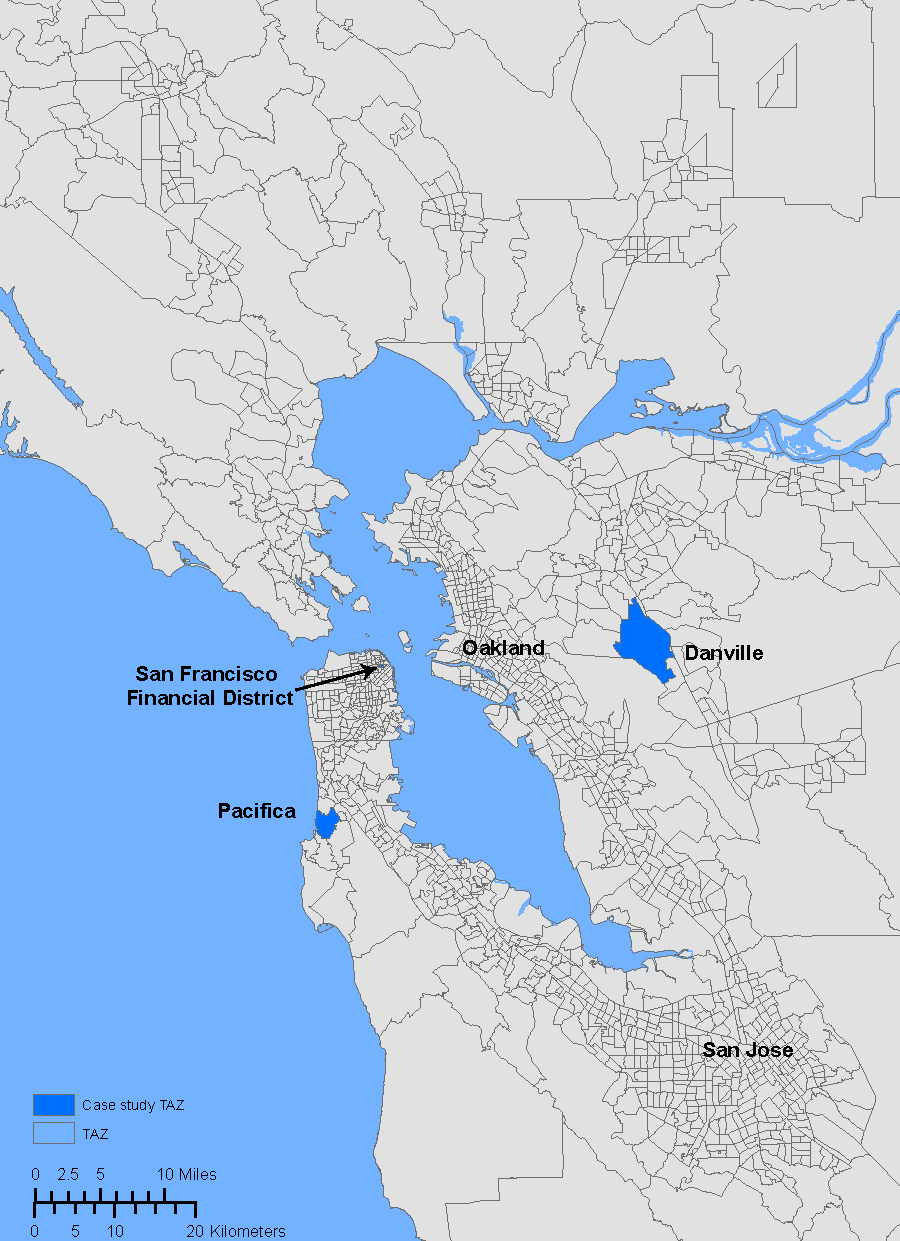
\includegraphics[width=4.5in]{../FIGS/equity_case.pdf} 
\caption{Study area: San Francisco Bay Area, CA with specific travel analysis zones (TAZs) used in the case study marked in blue.}
\label{fig:equity_study_area}
\end{figure}

\subsection{Case study overview}
We focus on the San Francisco Bay Area, a seismically-active region, to illustrate our approach (Figure~\ref{fig:equity_study_area}). The area follows a polycentric metropolitan form, with San Francisco as the primary center and other jobs  concentrated in suburban centers, such as Silicon Valley~\cite{cervero_polycentrism_1997}. The region has a wide array of trip patterns for mandatory and non-mandatory trips. Furthermore, trip times and routes vary greatly depending on travel preferences and workplace locations~\cite{cervero_polycentrism_1997}. Thus,  we might expect noticeable disparities between households in the risk of travel time delays due to earthquakes. 

This analysis considers the complex web of roads and transit networks of the case study area. The roads are modeled by a directed graph $G = (V, E)$, where $V$ is a finite set of vertices representing intersections, and the set $E$, whose elements are edges representing road links, is a binary relation on $V$. In this model, $(|V|, |E|)$ = (11,921, 32,858) including centroidal links and $(|V|, |E|)$ = (9,635, 24,404) without. Centroidal links do not correspond to particular physical roads but instead capture more subtle travel flows, such as  from outside the study area or the flow of people to and from some minor local roads. We also in 43 transit networks, as detailed in~\cite{miller_seismic_2014}.

We  model damage from ground shaking intensity to a set of 1743 highway bridges impacting the road and some transit networks, with data provided by the California Department of Transportation (Caltrans), and 1409 structures impacting the rapid transit network, BART, with data provided by that agency. We refer readers to~\cite{miller_seismic_2014} for more details about matching these structures, hereafter called components, to the relevant road and transit networks. 
%
% that represent the regional seismic hazard including events arising from the background seismicity which is not considered in the earlier study [18]. Table I lists pertinent information of these 50 scenario earthquakes.


\begin{sidewaysfigure}
\centering
\includegraphics[width=\textwidth]{../FIGS/Mahalia_four_pannels204v5_cropped.pdf} %methods_Mahalia_four_pannels204v3.png} 
\caption{Illustration of the risk framework for one earthquake event including a) One-second spectral acceleration  (ground-motion intensity) map with earthquake rupture, b) bridge (component) damage map, c) map of travel time increase (network-performance measure) values, and d) map of accessibility values averaged over all market segments by travel analysis zone (TAZ).}
\label{fig:four_steps}\end{sidewaysfigure}

\subsection{Ground-motion intensity maps}
\subsubsection{Theory}
We now describe how to produce a set of maps with ground-motion intensity realizations at each location of interest, and corresponding occurrence rates that reasonably capture the joint distribution of the ground-motion intensity. First, we generate $Q$ earthquake scenarios from a seismic source model. The seismic source model specifies the rates at which earthquakes of specified magnitudes, locations, and faulting types will occur. This set of earthquake scenarios is comparable to a stochastic event catalogue in the insurance industry.

Second, for each earthquake scenario in the seismic source model, we use an empirical ground-motion prediction equation (GMPE)~\cite[e.g.,][]{boore_ground-motion_2008%,abrahamson_summary_2008,chiou_nga_2008,campbell_nga_2008
} to model $Y$, the resulting intensity measure at each location of interest. %~\cite[e.g.,][]{foulser-piggott_predictive_2012}. %e.g., Foulser-Piggott and Stafford 2011). The GMPE predicts the mean of the log ground-motion intensity, $\overline{\ln Y (M_q, R_{iq}, V_{s30,i}, \ldots) }$ and ground-motion intensity within- and between-event residual standard deviations, which are denoted by \gls{sigma}$_{iq}$ and \gls{tau}$_q$ respectively, for the $i^{th}$ site where $i = 1, \ldots, $\gls{n} in the $q^{th}$ earthquake scenario where \gls{q}$=1, \ldots, $\gls{Q}, $M_q$ is the moment magnitude of the $q^{th}$ scenario, $R_{iq}$ is the closest horizontal distance from the surface projection of the fault plane to location $i$, and \gls{V_{s30,i}} is the average shear wave velocity down to 30$m$ at the $i^{th}$ location. 

Then, for each of the $Q$ earthquake scenarios, we sample $b$ realizations of the spatially-correlated ground-motion intensity residual terms~\cite[e.g.,][]{han_probabilistic_2012}. 
%Readers are referred to \cite{han_probabilistic_2012} for a survey of sampling methods.  
Once residuals are sampled, the total log ground-motion intensity ($Y$) is computed as 

\begin{equation}
\ln Y_{ij} = \overline{\ln Y (M_j, R_{ij}, V_{s30,i}, \ldots) }+ \sigma_{ij} \epsilon_{ij} + \tau_j \eta_j
\label{eq:GMPEmet}
\end{equation}
where $j$ is the ground-motion intensity map index ($j = 1, \ldots, m$ where $m = Q \times b$), $\epsilon_{ij}$ is the normalized within-event residual in $\ln Y$ representing location-to-location variability and $\eta_j$ is the normalized between-event residual in $\ln Y$ and the other parameters are defined above. Both $\epsilon_{ij}$ and $\eta_j$ are normal random variables with zero mean and unit standard deviation. The vector of $\epsilon_{ij}$ can be modeled by a spatially-correlated multivariate normal distribution~\cite[e.g.,][]{jayaram_correlation_2009} %Boore et al. 2003; Wang and Takada 2005; Goda and Hong 2008; Jayaram and Baker 2009 
and the $\eta_j$ by a standard univariate normal distribution. 

The result is a set of $m$ ground-motion intensity maps (e.g., Figure~\ref{fig:four_steps}{(a)}). Since we simulate an equal number ($b$) of ground-motion intensity maps per earthquake scenario, the annual rate of occurrence for the $j^{th}$ ground-motion intensity map is the original rate of occurrence of the earthquake scenario, divided by $b$. We denote the rate associated with the $j^{th}$ ground-motion intensity map as $w_j$.  

\subsubsection{Implementation}
To generate a stochastic catalog of ground-motion intensity maps, we use the OpenSHA Event Set Calculator~\cite{field_opensha:_2003}. This software outputs the mean, $\overline{\ln Y_{ij}}$, and standard deviation values, $\sigma_{ij}$ and $\tau_j$, for all locations of interest for a specified seismic source model and ground-motion prediction equation, which are needed inputs for Equation~\ref{eq:GMPEmet}. The intensity measure is the 5\%-damped pseudo absolute  spectral acceleration ($Sa$) at a period $T=1s$, which is the required input to the fragility functions below. This spectral acceleration value represents the maximum acceleration over time  that a linear oscillator with 5\% damping and a period of 1 second will experience from a given ground motion. We calculate these values at each component location (bridges and other structures). Using one ground-motion intensity measure per component is a common simplification of the time-varying acceleration dynamics~\cite[e.g.,][]{shinozuka_effect_2003,jayaram_efficient_2010} that may have lower errors for components with a natural period near 1 second as opposed to long-span bridges.
%In other words, we follow the standard practice of using one ground-motion intensity measure per component, which is a simplification of the true dynamics involving more dependence on the acceleration time histories, spatial differences in acceleration for a component (particularly long-span bridges), and 
We use the UCERF2 seismic source model~\cite{field_uniform_2009}, Wald and Allen topographic slope model for the the shear wave velocity $V_{s30,i}$~\cite{wald_topographic_2007}, and the Boore and Atkinson \cite{boore_ground-motion_2008} ground-motion prediction equation.   
%Using this seismic source model, which is then discretized into a list of faults and a stratified list of magnitudes and rupture locations for each, we obtain a set of 2110 earthquake events on all active faults, each with an annual occurrence rate greater than or equal to $10^{-5}$ . 
We simulate the ground-motion intensity maps by combining the mean terms from the Event Set Calculator and spatially-correlated residual terms of the ground-motion intensity  (using~\cite{jayaram_correlation_2009}) according to the basic ground-motion model  (eq.~\ref{eq:GMPEmet}). 

%, Equation~\ref{eq:GMPEmet}. 


\subsection{Damage maps}
\subsubsection{Theory}
Calculating network performance risk requires assessing the structural damage of relevant components after future earthquakes. The link between ground-motion intensity and structural damage is often provided by \emph{fragility functions}. Fragility functions express $P(DS_i \geq ds_{\varsigma} | Y_{ij} = y)$. We assume one component, such as a bridge, per site location, so we will identify both components and site locations via the index $i$. Using that notation, $DS_i$ is a discrete random variable whose value represents the damage state for the $i^{th}$ component and $ds$ is a damage state threshold of interest. The damage state is conditioned on a realization, $y$, of the random variable $Y_{ij}$, the ground-motion intensity at the $i^{th}$ site and $j^{th}$ ground-motion intensity map. Researchers have calibrated fragility functions using historical post-earthquake data~\cite[e.g.,][]{basoz_enhancement_1999}, experimental and analytical results~\cite[e.g.,][]{ramanathan_next_2012}, hybrid approaches, and expert opinion. Other work has investigated correlated damage states~\cite[e.g.,][]{lee_uncertainty_2007}. 
%It is possible to sample the damage states from  a joint distribution that includes correlation, such as due to similarities in design or construction practices~\cite[e.g.,][]{lee_uncertainty_2007}. 

By sampling a damage state for each component, with probabilities obtained from the fragility functions given the ground-motion intensity, we produce a damage map (e.g., Figure~\ref{fig:four_steps}{(b)}). The damage map has a realization of the damage state of each relevant component. This sampling process can be repeated multiple times to simulate multiple damage maps per ground-motion intensity map. For example, if equal numbers of damage maps are sampled per ground-motion intensity map ($c$ damage maps per ground-motion intensity map), the weight of the $j'^{th}$ damage map should be adjusted accordingly to $w_{j'}$, where $w_{j'} = \frac{w_j}{c}$, and $j' = 1, \ldots, J$. 

%These damage maps are directly mapped to the functionality of elements of the network. 
\emph{Functional percentage} relationships link the component damage to the functionality of network elements.  For example, in a road network, when a bridge collapses, the traffic flow capacity of the road it carries and it crosses can be modeled as reduced to zero. These relationships are typically derived from a combination of observation and expert opinion, often due to data scarcity~\cite{werner_redars_2006}. Furthermore, the relationships are typically deterministic for a certain component damage state and restoration time~\cite{werner_redars_2006}. Thus, in this paper, each damage map corresponds to a functionality state for every element of the network.

\subsubsection{Implementation}
\paragraph{Component damage}


%We do not include other types of network component failures such as liquefaction in this study.
For the case study, we use fragility functions of the following form to provide the link between ground-motion shaking and component damage:
\begin{equation}
%$P(DS \geq ds_s | Y = y_{ij}, i)$
P(DS_i \geq ds_\varsigma |Y_{ij} = y) = \Phi \left( \frac{\ln y - \lambda_{\varsigma, i}}{\xi_{\varsigma,i}} \right),
\label{eq:dsfull}
\end{equation}
where $\Phi$ is the standard normal cumulative distribution function, $\lambda_{\varsigma,i}$ and $\xi_{\varsigma,i}$ are respectively the mean and standard deviation of the $\ln Y_{ij}$ value necessary to cause the $\varsigma^{th}$ damage state to occur or be exceeded for the $i^{th}$ component, and the other variables are defined above. By using the previous equation and the inverse method, we can sample realizations of component damage states for a given ground-motion intensity.
%
%
%where $DS_i$ is a discrete random variable, whose value represents the damage state, $s$, for each bridge index $i$. $\Phi$ is the standard normal cumulative distribution function and $\lambda_{s,i}$ and $\xi$ are respectively the mean and standard deviation of the $\ln Y$ value necessary to cause the $s^{th}$ damage state to occur or be exceeded. $y_{i,j}$ is the spectral acceleration value that the bridge experiences for the $j^{th}$ ground-motion intensity map. 

The California Department of Transportation (Caltrans) provided the fragility function values $\lambda_{\varsigma,i}$ and $\xi_{\varsigma,i}$ used in this study for the highway components in summer 2012, which was last updated in 2007 and includes various retrofitted bridges~\cite{caltrans_caltrans_2013}. The $\lambda_{\varsigma,i}$ values are based on component characteristics including number of spans and age as detailed in \cite{basoz_enhancement_1999}. The $\xi_{\varsigma,i}$ values are given as a constant. The BART seismic safety group provided the  fragility function values $\lambda_{\varsigma,i}$ and $\xi_{\varsigma,i}$ used in this study for the BART-related components for the state of the network in summer 2012. Data is available for the aerial structures, primarily in the East Bay, but not tunnels. The BART fragility function values correspond to the safety performance goals under the recent retrofit program~\cite{bechtel/hntb_team_design_2008}. The numbers are comparable to the Caltrans fragility data. For the BART components, however, $\xi_{\varsigma,i}$, the standard deviation of the $\ln Sa$ value necessary to cause the extensive damage state to occur or be exceeded, varies depending on the component. Both sets of fragility functions are based on the assumption that damage can be reasonably accurately estimated by the ground motion intensity at each site independently, and that the damage state can be reasonably estimated by an analytical model considering a single ground-motion intensity measure.  In addition, the fragility curves do not directly consider the effects of degradation. Current work is ongoing to refine these assumptions~\cite[e.g.,][]{ramanathan_next_2012,kurtz_time-varying_2014,ghosh_seismic_2013}. 

%Caltrans also provided other component properties such as length, construction year, construction materials, out-to-out distance (the maximum distance in the perpendicular direction to traffic flow), number of spans, and average daily traffic flow). Similarly, Caltrans provided estimates for bridge replacement costs in current (2014) USD: 175  per square foot for construction and 10  per square foot for demolition of the damaged bridge~\cite{pugh_construction_2012}. 


%\begin{figure}[h!]
%\centering
%\includegraphics[width=6in]{../FIGS/bridges_adt_histlong.eps} 
%\caption{Histogram of the average daily traffic counts for the road component (bridge) dataset from Caltrans.}
%\label{fig:adt}
%\end{figure}
%
% using the method detailed in \cite{basoz_enhancement_1999} based on The structural capacities of individual bridges are modeled as uncorrelated.

Per ground-motion intensity map, we sample one damage map (e.g., Figure~\ref{fig:four_steps}{(b)}), which has a realization of the component damage state at each component location according to the fragility function (eq.~\ref{eq:dsfull}). The provided fragility functions do not consider correlation of the structural capacities, but other models could be used~\cite[e.g.,][]{lee_uncertainty_2007}.

\paragraph{Transit network damage}
\label{sec:transitDamage}
Each of the 43 transit systems we considered will be impacted differently. For Caltrain, conversations with managers suggest that given that there is one shared track system, the system would either be fully operational or  not at all. Similarly, managers suggested modeling the VTA system as fully functional or not. Depending on where the BART train cars are when the earthquake strikes, the agency could accommodate different emergency plans. However, BART representatives suggested considering that if any part of a route is damaged, the entire corresponding route would not be operational (but other routes on different tracks might be still operational).  In other words, each BART route as well as the Caltrain and VTA routes are each a weakest-link system,  so the failure of a single component  will cause the route to be non-operational. We modeled the ferry systems as fully functioning for all earthquake events. For all earthquake events including the baseline, trans-bay and cross-county bus lines were discontinued, but main lines in urban areas as well as other local bus networks were maintained per recommendations from the MTC, though they may face delays due to modeled traffic congestion. 

\paragraph{Road network damage}

%For this case study, we represent the road network by a directed graph $G = (V, E)$, where $V$ is a finite set of vertices representing intersections and the set $E$, whose elements are edges representing road links, is a binary relation on $V$. This study considers the Metropolitan Transportation Commission (MTC) \emph{Travel Model One} (version 0.3) of the San Francisco Bay Area transportation network where $(|V|, |E|) = (11921, 32858)$ including centroidal links and $(|V|, |E|) = (9635, 24404)$ without. The model includes both highways and main local roads as well as the relevant trip demand data. 
%The travel origin-demand matrix for the latest run version, 2010\_03\_YYY, is from the MTC. The MTC travel origin-destination matrix is divided into the 4362 subzones of the 1454 traffic analysis zones (TAZs) based on population density covering the 9-county San Francisco Bay Area. We also use an aggregated version of the origin-destination matrix using 34 super districts.

The damage state of each component maps directly to the traffic capacity on associated road segments. We use a functional percentage relationship to compute the traffic capacity of relevant road segments. Based on discussions with Caltrans, we consider travel conditions one week after an earthquake, since it is a critical period for decision making. For example, one week after most events, bridges should have been inspected and surface damage should be repaired, but major reconstruction would not have yet begun. According to our functional percentage relationship, at this point in time, the components have one of two classes of functionality, zero traffic capacity and full traffic capacity~\cite{werner_redars_2006}. We can thus summarize the component damage using two damage states $ds_s$, $ds_{damaged}$ and $ds_{functional}$, which correspond to the common HAZUS \emph{extensive} or \emph{complete} damage states and the \emph{none}, \emph{slight}, or \emph{moderate} damage states respectively~\cite{werner_redars_2006}. Thus, the functional percentage relationship assigns zero traffic capacity on road segments that have at least one component in the $ds_{damaged}$ damage state, and full traffic capacity otherwise.  We do not consider network damage from sources other than main structural damage from ground shaking, such as tunnel displacement or liquefaction, but the framework allows including such considerations. 
%In the discussion below, we consider a set of 113,940 damage maps, which correspond to 2110 scenarios, 3 ground-motion intensity maps per scenario, and 18 damage maps per ground-motion intensity map. 




\subsection{Network performance}
\subsubsection{Theory}
The final step for the event-based risk analysis is to evaluate the network performance measure, $X$. For this application, we consider a metric popular in urban planning, \emph{mode-destination accessibility change}~\cite[e.g.,][]{geurs_accessibility_2004,kockelman_travel_1997,waddell_incorporating_2002}  (e.g., Figure~\ref{fig:four_steps}{(d)}). Mode-destination accessibility, hereafter referred to as accessibility, measures the distribution of travel destination opportunities weighted by the composite utility of all modes of travel to those destinations, i.e., the ease of someone getting to different destinations weighted by how desirable those destinations are~\cite{handy_measuring_1997,niemeier_accessibility:_1997}. The utility function for the mode-destination choice may be estimated using a multinomial random utility model where the logsum represents the accessibility value~\cite{manski_structural_1981,handy_measuring_1997,niemeier_accessibility:_1997}. Namely, accessibility for a particular agent $a$ is
\begin{equation}
Acc_a = \ln \left[ \sum_{\forall \in C_a} \exp (V_{a(c)}) \right],
\label{eq:acc}
\end{equation}
where $V_{a(c)}$ is the utility of the $c^{th}$ choice for the $a^{th}$ person for $a = 1, \ldots, A$, and $C_a$ is the choice set for the $a^{th}$ person~\cite{handy_measuring_1997}. Choices refer to travel destinations and the mode of travel (driving, walking, bus, etc.). The units are a dimensionless quantity, $utils$. As an extension, the accessibility values from the previous equation can be converted into equivalent time and dollar amounts using \emph{compensating variation} for cost-benefit studies; for the case study, 0.0134 $utils$ (generic measure of utility) equals the value of one minute per day~\cite{niemeier_accessibility:_1997,small_applied_1981,ory_personal_2013} and we conservatively value one hour of time as approximately \$15~\cite{united_states_department_of_transportation_revised_2011}. In other words, one $util$ is worth approximately \$20 per person per day based on these assumptions. With nearly 7 million people in the region, even small changes in $utils$ lead to large economic losses. Since accessibility measures how easily people can get to the destinations they desire, accessibility is used as one of the measures of human welfare~\cite[e.g.,][]{niemeier_accessibility:_1997}.

%Furthermore, we will consider consider the fixed-demand \emph{travel time increase} performance measure~\cite[e.g.,][]{jayaram_efficient_2010,han_probabilistic_2012}. Travel time increase is the change in the cumulative change in the amount of time every trip takes during a given time period from the pre-earthquake to post-earthquake conditions (one week post-earthquake). An example of this travel time increase for each road segment is shown in Figure~\ref{fig:four_steps}{(c)}.

%Finally, we estimate the annual rate, $\lambda$, of exceeding some threshold of network performance. This rate is estimated by summing the occurrence rates of all damage maps in which the performance measure exceeds the threshold: 
%\begin{equation}
%\lambda_{X \geq x} = \sum_{j'=1}^{J} w_{j'} \mathbbm{I}(X_{j'}\geq x)
%\label{eq:exceedance}
%\end{equation}
%where $x$ is an accessibility value threshold of interest and $X_{j'}$ is the accessibility value realization for the $j'^{th}$ damage map. The variable $w_{j'}$ is the occurrence rate of the $j'^{th}$ damage map.% ($w_j = \frac{w_j}{c}$ where $c$ is the number of damage map realizations per ground-motion intensity map). 
%%The function $\mathbbm{I}$ is an indicator function that evaluates to 1 if the argument, $x_j' \geq x$, is true and 0 otherwise. 
%The indicator function $\mathbbm{I}$  evaluates to 1 if the argument, $X_{j'} \geq x$, is true, and 0 otherwise.
%By evaluating $\lambda$ at different threshold values, we derive an exceedance curve, e.g., Figure~\ref{fig:acc_by_TAZ_and_income}). 

Once the accessibility network performance measure is computed for each damage map, we aim to estimate the exceedance rate of different levels of performance. The annual rate, $\lambda$, of exceeding some threshold of network performance is estimated by summing the occurrence rates of all damage maps in which the performance measure exceeds the threshold: 
\begin{equation}
\lambda_{X \geq x} = \sum_{j'=1}^{J} w_{j'} \mathbbm{I}(X_{j'}\geq x)
\label{eq:exceedance}
\end{equation}
where $x$ is an accessibility value threshold of interest and $X_{j'}$ is the accessibility value realization for the $j'^{th}$ damage map. The variable $w_{j'}$ is the occurrence rate of the $j'^{th}$ damage map.% ($w_j = \frac{w_j}{c}$ where $c$ is the number of damage map realizations per ground-motion intensity map). 
%The function $\mathbbm{I}$ is an indicator function that evaluates to 1 if the argument, $x_j' \geq x$, is true and 0 otherwise. 
The indicator function $\mathbbm{I}$  evaluates to 1 if the argument, $X_{j'} \geq x$, is true, and 0 otherwise. By evaluating $\lambda$ at different threshold values, we derive an exceedance curve (e.g., Figure~\ref{fig:acc_by_TAZ_and_income}). 

%First, we assign travel demand to the transportation network. Then, we compute the cumulative travel time for the $j'^{th}$ network damage map over all trips \gls{T}, which is the set of trips between the different demand origin and destinations chosen when travel demand is assigned to the transportation network. 
%
%Before calculating travel time, we first formalize the idea of a path. For a trip from an origin \gls{s} to a destination \gls{t}, the path is \gls{p}$(s,t) = (v_0, v_1, \dots , v_{\text{\gls{kappa}}})$ where each $v \in V$ are consecutive vertices, and there are \gls{kappa} vertices in the path. In general, the weight of a path, \gls{w_z}, is
%\begin{equation}
%w_z(p) = \sum_{i=1}^{\kappa} z(v_{i-1}, v_i)
%\label{eq:path_weight}
%\end{equation}
%where \gls{z} is the edge weight between two vertices for the general case.  
%%For travel time, for example, \gls{z}, is the congested travel time for that edge, \gls{t_a}.
%%Note that for travel time, the edge weight metric, \gls{z}, is the congested travel time for that edge, \gls{t_a}.
%
%Aggregating these values over all trips and defining  \gls{z} as the congested travel time for an edge, \gls{t_a}, we find the total travel time as follows:
%\begin{equation}
%TT = \sum_{p \in T}  w_z(p),
%\label{eq:tt}
%\end{equation}
%where the edge weight metric, \gls{z}, is the congested travel time, \gls{t_a}.
%The travel time increase is defined as \gls{TT}$_j - TT_{\text{base}}$, which is the difference in travel time between the $j'^{th}$ network damage map and the base case (undamaged). 
%%We implement travel time increase in NetworkX, as part of our efficient travel model. 
%
%
%
%Using the efficient traffic model, we first assign travel demand to the transportation network with the iterative traffic assignment (ITA) method~\cite{chen_network_1991} that assigns travel demand iteratively. We implement ITA according to the recommendations of~\cite{wang_understanding_2012}, where the original demand matrix is divided into four parts, with 40\%, 30\%, 20\%, and 10\% respectively of the total trips. To begin, the first part of the trips are assigned using Dijkstra's algorithm~\cite{dijkstra_note_1959} to find shortest paths where the non-negative edge weights are the free-flow travel time (\gls{t_f}). The resulting link flows (\gls{q_a}) are recorded for each link. Then, we update the travel time (\gls{t_a}) on each link according to the commonly-used formula,
%\begin{equation}
% t_a = t_f \left(1 + 0.15 \left( \frac{q_a}{c_f}\right)^{4}\right),
% \end{equation}
% where \gls{c_f} is the flow capacity of the link~\cite{bureau_of_public_roads_traffic_1964}. 
% 
%Then, using these new congested travel time values (\gls{t_a}) as the edge weights, we use Dijkstra's algorithm to assign the second part of the trips. We repeat this approach until we have assigned all four parts of the trips. This ITA method has been shown to effectively estimate driver behavior because intuitively it captures drivers' choices of routes based on what traffic situation they currently see~\cite{wang_understanding_2012} and to be roughly consistent with results from the commonly-used User Equilibrium (UE) method~\cite{wang_understanding_2012,beckmann_studies_1956}, which is used in one stage of each iteration of the high-fidelity model. The main difference is that the UE method assumes that people all have perfect knowledge of the system and make the ideal choice individually, whereas the ITA method corresponds to people seeing some congestion on the road and choosing a route that seems fastest at that time. Finally, the actual fixed-demand travel time calculation is to sum the products of the new edge flow (\gls{q_a}) and congested travel time (\gls{t_a}) values over all edges. This is equivalent to the summing up the congested travel times over all edges in all paths (Equation~\ref{eq:tt}). The procedure is summarized in Miller 2014~\cite{miller_seismic_2014}.

%We will consider various network performance measures, each of which is a scalar quantity per damage map.  
%%something about transportation
%For road networks, two common performance measures are connectivity~\cite{basoz_bridge_1995,rokneddin_bridge_2013} and flow capacity~\cite{lee_post-hazard_2011}.  In order of increasing general computational cost, other measures to capture road network performance include the percentage of bridges damaged, weighted-shortest path between locations of interest \cite{chang_measuring_2001}, fixed-demand travel-time~\cite{stergiou_treatment_2006,shiraki_system_2007,jayaram_efficient_2010,han_probabilistic_2012}, morning or evening peak commute time, economic impacts from increased travel time and bridge repairs \cite{stergiou_treatment_2006}, and mode-destination accessibility~\cite{handy_measuring_1997}.  Fixed-demand travel time delay and its variants have become particularly popular in current literature (e.g., Figure~\ref{fig:sample_pipeline}{(c)}).
%%something about power
%For power networks, connectivity is also a common network performance measure~\cite{duenas-osorio_seismic_2007}. Recently, power network researchers have introduced other measures such as serviceability ratio~\cite{adachi_serviceability_2008}, power system flow \cite{winkler_performance_2010}, and recovery time of the electrical network~\cite{shinozuka_seismic_2007}.
%%something about water
%Researchers have also used connectivity to measure the reliability of water networks with alternative measures including flow capacity, entropy-based measures, nodal demands, and the total number of component failures system-wide~\cite{romero_seismic_2010,hernandez-fajardo_sequential_2011,goulter_analytical_1995}.
%\subsubsection{Implementation}
%

%\subsection{Model description}
%We introduce two models to estimate the performance of the transportation network: a high-fidelity model and an efficient model.
\subsubsection{Implementation}
We compute accessibility using  \emph{Travel Model One} (version 0.3), an activity-based model used by the Metropolitan Transportation Commission (MTC), the local metropolitan planning organization (MPO)~\cite{erhardt_mtcs_2012}. It represents the full road network as well as the public transit networks, biking, and walking. Travel demand data consists of the locations of different households in the case study area, their destination preferences and utilities, their number of vehicles, and their income and other demographic data~\cite{erhardt_mtcs_2012,ory_personal_2013}. More details can be found in~\cite{waddell_urbansim:_2002}. This data was collected by the MTC from surveys and census information. We assume that the distributions of travel preferences do not change after an earthquake, although the actual destinations and trips may vary. For example, if a trip takes a very long time after a simulated earthquake, it is less likely that a person will choose to take the trip. The result is a \emph{variable} travel demand model. This model uses a combination of Java code called CT-RAMP~\cite{davidson_ct-ramp_2010}, and the Citilabs Cube Voyager and Cube Cluster software programs, which are part of a leading commercial software suite for transportation planning~\cite{erhardt_mtcs_2012}. This model differs from previous representations of this network~\cite[e.g.,][]{jayaram_efficient_2010,wakabayashi_network_1992}, since it includes not only major roads but also local roads and transit lines. We have provided further details about computing mode-destination accessibility using this high-fidelity model in~\cite{miller_seismic_2014}.

This analysis considers 40 interesting and hazard-consistent events, as defined by 40 sets of ground-motion intensity maps, damage maps, accessibility performance measure realizations, and corresponding annual rates of occurrence. We selected this set of events with the optimization-based procedure introduced in~\cite{miller_ground-motion_2014}. Readers are referred to~\cite{miller_seismic_2014} for more details about this set of events. 

In the following sections, we first compare region-wide results, and then focus on particular characteristics of three communities. Finally, we discuss generalizable trends.
%We compute accessibility by xxxx $$

%\subsubsection{Efficient travel model description}
%The efficient model represents the full road network by the directed graph $G$ and, for simplicity, does not include the transit network. The edge properties we model are flow capacity ($c_f$) in vehicles per hour, free-flow travel time ($t_f$) in minutes, congested travel time ($t_a$), flow  ($q_a$) in vehicles per hour, and distance/length ($d_0$) in miles. The efficient model is implemented in Python using a software package intended for social network analysis, NetworkX~\cite{hagberg_exploring_2008}, which we have leveraged for this new application. The daily travel origin-demand matrix, 2010\_03\_YYY, for vehicle traffic only is from the MTC and is based on travel surveys, census information, and compared with sensor data~\cite{erhardt_mtcs_2012}. It is based on weekday, non-earthquake travel demand. In other words, this model assumes a fixed demand and a single transportation mode (driving), two assumptions relaxed in the high-fidelity model case above. For this efficient model, we use a version of the daily travel origin-destination matrix that is aggregated to data between all permutations of the 34 superdistricts of the San Francisco Bay Area. Superdistricts are based on population size and are zones used by local authorities in a few regions, including the San Francisco Bay Area, for traffic analysis and urban planning. Each superdistrict contains multiple travel analysis zones (TAZs) that represent a more granular version of superdistricts; sub-zones of the TAZs are used in the high-fidelity model. For each superdistrict, we model one centroid as a supernode, which refers to a dummy node with directed edges to a few actual nodes in the network within the target area~\cite{lim_seismic_2014}. 
%%Figure~\ref{fig:centroids}{(a)} illustrates the supernodes for superdistricts 1 and 2. 
%Supernodes are advantageous for this application, because they relatively accurately capture the diffuse nature of travel demand. In contrast, if all superdistrict travel demand is inputted at one node per superdistrict with one outgoing link each, the model would be unrealistically sensitive to damage on this one link.
%%Results using supernodes are more realistic because without supernodes, and if there is only one link from where superdistrict travel demand is inputted and it connects to a major roads and a bridge is damaged on this path, the model would think that these people are disconnected from the network. In reality, there would likely be other local roads. 
%Then, to convert from the daily travel origin-demand matrix data to hourly values, we use 5.3\% of the daily travel demands, which is based on the recorded data from \cite{wang_understanding_2012}, to represent one hour of morning travel demands during the 6-10am commute period. Again, this assumes fixed travel demand. We have provided further details about computing the fixed-demand travel time using the efficient model in~\cite{miller_seismic_2014}.
%\begin{figure}[ht]
%\centering
%\includegraphics[width=5.5in]{FIGS/methods_super.pdf} 
%\caption{Map of 34 superdistricts.}
%\label{fig:superdistricts}
%\end{figure}
%
%\begin{figure}[ht]
%\centering
%\includegraphics[width=6in]{FIGS/methods_superNode.eps} 
%\caption{Map of supernodes for a) local flow between superdistrict one (SD1) \emph{supernode} and superdistrict two (SD2)  \emph{supernode}, and b) San Francisco \emph{area supernode} to Oakland  \emph{area supernode}. Some nodes, representing road intersections, in the road graph G connect to or from superdistrict supernodes. Some superdistrict supernodes connect to or from area supernodes.}
%\label{fig:centroids}
%\end{figure}

%We compute the fixed-demand travel time by xxxx $$

%\subsubsection{Event set selection using optimization}
%From a large set of ground-motion intensity maps and damage maps, we choose a set of forty maps, using the optimization procedure we proposed in Miller and Baker~\cite{miller_ground-motion_2014}; we chose the fixed-demand travel time delay as the proxy metric, because it is related to travel time delays expected in the high-fidelity model. We then use the high-fidelity model to predict the transportation network impacts of the forty pairs of ground-motion intensity and damage maps. The outcome is forty sets of results for the target performance metric, mode-destination accessibility. Each accessibility value has a corresponding annual rate of occurrence.


%\clearpage
%\section{Risk framework}
%\label{sec:accGeo}
%\begin{figure}
\centering
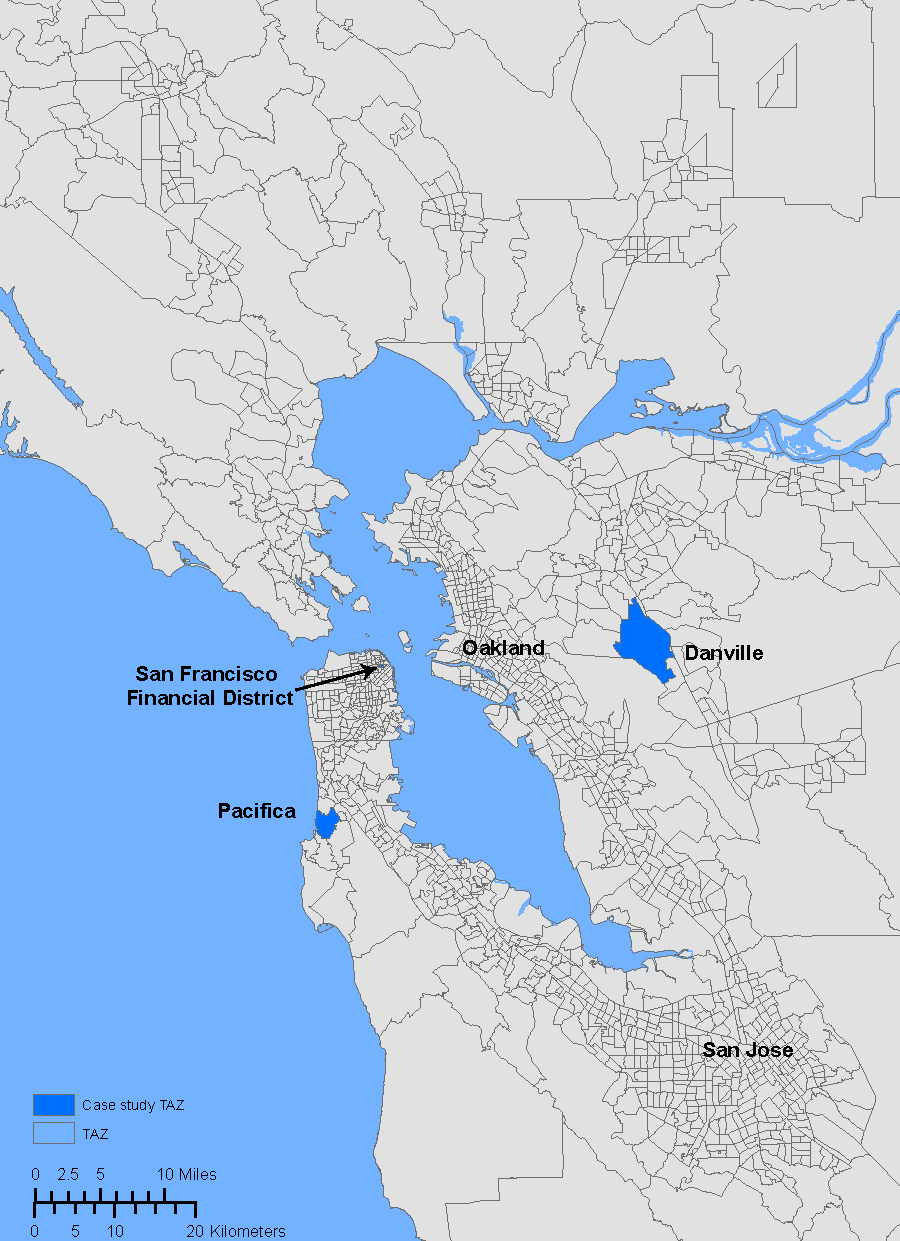
\includegraphics[width=4.5in]{../FIGS/equity_case.pdf} 
\caption{Study area: San Francisco Bay Area, CA with specific travel analysis zones (TAZs) used in the case study marked in blue.}
\label{fig:equity_study_area}
\end{figure}

\subsection{Case study overview}
We focus on the San Francisco Bay Area, a seismically-active region, to illustrate our approach (Figure~\ref{fig:equity_study_area}). The area follows a polycentric metropolitan form, with San Francisco as the primary center and other jobs  concentrated in suburban centers, such as Silicon Valley~\cite{cervero_polycentrism_1997}. The region has a wide array of trip patterns for mandatory and non-mandatory trips. Furthermore, trip times and routes vary greatly depending on travel preferences and workplace locations~\cite{cervero_polycentrism_1997}. Thus,  we might expect noticeable disparities between households in the risk of travel time delays due to earthquakes. 

This analysis considers the complex web of roads and transit networks of the case study area. The roads are modeled by a directed graph $G = (V, E)$, where $V$ is a finite set of vertices representing intersections, and the set $E$, whose elements are edges representing road links, is a binary relation on $V$. In this model, $(|V|, |E|)$ = (11,921, 32,858) including centroidal links and $(|V|, |E|)$ = (9,635, 24,404) without. Centroidal links do not correspond to particular physical roads but instead capture more subtle travel flows, such as  from outside the study area or the flow of people to and from some minor local roads. We also in 43 transit networks, as detailed in~\cite{miller_seismic_2014}.

We  model damage from ground shaking intensity to a set of 1743 highway bridges impacting the road and some transit networks, with data provided by the California Department of Transportation (Caltrans), and 1409 structures impacting the rapid transit network, BART, with data provided by that agency. We refer readers to~\cite{miller_seismic_2014} for more details about matching these structures, hereafter called components, to the relevant road and transit networks. 
%
% that represent the regional seismic hazard including events arising from the background seismicity which is not considered in the earlier study [18]. Table I lists pertinent information of these 50 scenario earthquakes.


\begin{sidewaysfigure}
\centering
\includegraphics[width=\textwidth]{../FIGS/Mahalia_four_pannels204v5_cropped.pdf} %methods_Mahalia_four_pannels204v3.png} 
\caption{Illustration of the risk framework for one earthquake event including a) One-second spectral acceleration  (ground-motion intensity) map with earthquake rupture, b) bridge (component) damage map, c) map of travel time increase (network-performance measure) values, and d) map of accessibility values averaged over all market segments by travel analysis zone (TAZ).}
\label{fig:four_steps}\end{sidewaysfigure}

\subsection{Ground-motion intensity maps}
\subsubsection{Theory}
We now describe how to produce a set of maps with ground-motion intensity realizations at each location of interest, and corresponding occurrence rates that reasonably capture the joint distribution of the ground-motion intensity. First, we generate $Q$ earthquake scenarios from a seismic source model. The seismic source model specifies the rates at which earthquakes of specified magnitudes, locations, and faulting types will occur. This set of earthquake scenarios is comparable to a stochastic event catalogue in the insurance industry.

Second, for each earthquake scenario in the seismic source model, we use an empirical ground-motion prediction equation (GMPE)~\cite[e.g.,][]{boore_ground-motion_2008%,abrahamson_summary_2008,chiou_nga_2008,campbell_nga_2008
} to model $Y$, the resulting intensity measure at each location of interest. %~\cite[e.g.,][]{foulser-piggott_predictive_2012}. %e.g., Foulser-Piggott and Stafford 2011). The GMPE predicts the mean of the log ground-motion intensity, $\overline{\ln Y (M_q, R_{iq}, V_{s30,i}, \ldots) }$ and ground-motion intensity within- and between-event residual standard deviations, which are denoted by \gls{sigma}$_{iq}$ and \gls{tau}$_q$ respectively, for the $i^{th}$ site where $i = 1, \ldots, $\gls{n} in the $q^{th}$ earthquake scenario where \gls{q}$=1, \ldots, $\gls{Q}, $M_q$ is the moment magnitude of the $q^{th}$ scenario, $R_{iq}$ is the closest horizontal distance from the surface projection of the fault plane to location $i$, and \gls{V_{s30,i}} is the average shear wave velocity down to 30$m$ at the $i^{th}$ location. 

Then, for each of the $Q$ earthquake scenarios, we sample $b$ realizations of the spatially-correlated ground-motion intensity residual terms~\cite[e.g.,][]{han_probabilistic_2012}. 
%Readers are referred to \cite{han_probabilistic_2012} for a survey of sampling methods.  
Once residuals are sampled, the total log ground-motion intensity ($Y$) is computed as 

\begin{equation}
\ln Y_{ij} = \overline{\ln Y (M_j, R_{ij}, V_{s30,i}, \ldots) }+ \sigma_{ij} \epsilon_{ij} + \tau_j \eta_j
\label{eq:GMPEmet}
\end{equation}
where $j$ is the ground-motion intensity map index ($j = 1, \ldots, m$ where $m = Q \times b$), $\epsilon_{ij}$ is the normalized within-event residual in $\ln Y$ representing location-to-location variability and $\eta_j$ is the normalized between-event residual in $\ln Y$ and the other parameters are defined above. Both $\epsilon_{ij}$ and $\eta_j$ are normal random variables with zero mean and unit standard deviation. The vector of $\epsilon_{ij}$ can be modeled by a spatially-correlated multivariate normal distribution~\cite[e.g.,][]{jayaram_correlation_2009} %Boore et al. 2003; Wang and Takada 2005; Goda and Hong 2008; Jayaram and Baker 2009 
and the $\eta_j$ by a standard univariate normal distribution. 

The result is a set of $m$ ground-motion intensity maps (e.g., Figure~\ref{fig:four_steps}{(a)}). Since we simulate an equal number ($b$) of ground-motion intensity maps per earthquake scenario, the annual rate of occurrence for the $j^{th}$ ground-motion intensity map is the original rate of occurrence of the earthquake scenario, divided by $b$. We denote the rate associated with the $j^{th}$ ground-motion intensity map as $w_j$.  

\subsubsection{Implementation}
To generate a stochastic catalog of ground-motion intensity maps, we use the OpenSHA Event Set Calculator~\cite{field_opensha:_2003}. This software outputs the mean, $\overline{\ln Y_{ij}}$, and standard deviation values, $\sigma_{ij}$ and $\tau_j$, for all locations of interest for a specified seismic source model and ground-motion prediction equation, which are needed inputs for Equation~\ref{eq:GMPEmet}. The intensity measure is the 5\%-damped pseudo absolute  spectral acceleration ($Sa$) at a period $T=1s$, which is the required input to the fragility functions below. This spectral acceleration value represents the maximum acceleration over time  that a linear oscillator with 5\% damping and a period of 1 second will experience from a given ground motion. We calculate these values at each component location (bridges and other structures). Using one ground-motion intensity measure per component is a common simplification of the time-varying acceleration dynamics~\cite[e.g.,][]{shinozuka_effect_2003,jayaram_efficient_2010} that may have lower errors for components with a natural period near 1 second as opposed to long-span bridges.
%In other words, we follow the standard practice of using one ground-motion intensity measure per component, which is a simplification of the true dynamics involving more dependence on the acceleration time histories, spatial differences in acceleration for a component (particularly long-span bridges), and 
We use the UCERF2 seismic source model~\cite{field_uniform_2009}, Wald and Allen topographic slope model for the the shear wave velocity $V_{s30,i}$~\cite{wald_topographic_2007}, and the Boore and Atkinson \cite{boore_ground-motion_2008} ground-motion prediction equation.   
%Using this seismic source model, which is then discretized into a list of faults and a stratified list of magnitudes and rupture locations for each, we obtain a set of 2110 earthquake events on all active faults, each with an annual occurrence rate greater than or equal to $10^{-5}$ . 
We simulate the ground-motion intensity maps by combining the mean terms from the Event Set Calculator and spatially-correlated residual terms of the ground-motion intensity  (using~\cite{jayaram_correlation_2009}) according to the basic ground-motion model  (eq.~\ref{eq:GMPEmet}). 

%, Equation~\ref{eq:GMPEmet}. 


\subsection{Damage maps}
\subsubsection{Theory}
Calculating network performance risk requires assessing the structural damage of relevant components after future earthquakes. The link between ground-motion intensity and structural damage is often provided by \emph{fragility functions}. Fragility functions express $P(DS_i \geq ds_{\varsigma} | Y_{ij} = y)$. We assume one component, such as a bridge, per site location, so we will identify both components and site locations via the index $i$. Using that notation, $DS_i$ is a discrete random variable whose value represents the damage state for the $i^{th}$ component and $ds$ is a damage state threshold of interest. The damage state is conditioned on a realization, $y$, of the random variable $Y_{ij}$, the ground-motion intensity at the $i^{th}$ site and $j^{th}$ ground-motion intensity map. Researchers have calibrated fragility functions using historical post-earthquake data~\cite[e.g.,][]{basoz_enhancement_1999}, experimental and analytical results~\cite[e.g.,][]{ramanathan_next_2012}, hybrid approaches, and expert opinion. Other work has investigated correlated damage states~\cite[e.g.,][]{lee_uncertainty_2007}. 
%It is possible to sample the damage states from  a joint distribution that includes correlation, such as due to similarities in design or construction practices~\cite[e.g.,][]{lee_uncertainty_2007}. 

By sampling a damage state for each component, with probabilities obtained from the fragility functions given the ground-motion intensity, we produce a damage map (e.g., Figure~\ref{fig:four_steps}{(b)}). The damage map has a realization of the damage state of each relevant component. This sampling process can be repeated multiple times to simulate multiple damage maps per ground-motion intensity map. For example, if equal numbers of damage maps are sampled per ground-motion intensity map ($c$ damage maps per ground-motion intensity map), the weight of the $j'^{th}$ damage map should be adjusted accordingly to $w_{j'}$, where $w_{j'} = \frac{w_j}{c}$, and $j' = 1, \ldots, J$. 

%These damage maps are directly mapped to the functionality of elements of the network. 
\emph{Functional percentage} relationships link the component damage to the functionality of network elements.  For example, in a road network, when a bridge collapses, the traffic flow capacity of the road it carries and it crosses can be modeled as reduced to zero. These relationships are typically derived from a combination of observation and expert opinion, often due to data scarcity~\cite{werner_redars_2006}. Furthermore, the relationships are typically deterministic for a certain component damage state and restoration time~\cite{werner_redars_2006}. Thus, in this paper, each damage map corresponds to a functionality state for every element of the network.

\subsubsection{Implementation}
\paragraph{Component damage}


%We do not include other types of network component failures such as liquefaction in this study.
For the case study, we use fragility functions of the following form to provide the link between ground-motion shaking and component damage:
\begin{equation}
%$P(DS \geq ds_s | Y = y_{ij}, i)$
P(DS_i \geq ds_\varsigma |Y_{ij} = y) = \Phi \left( \frac{\ln y - \lambda_{\varsigma, i}}{\xi_{\varsigma,i}} \right),
\label{eq:dsfull}
\end{equation}
where $\Phi$ is the standard normal cumulative distribution function, $\lambda_{\varsigma,i}$ and $\xi_{\varsigma,i}$ are respectively the mean and standard deviation of the $\ln Y_{ij}$ value necessary to cause the $\varsigma^{th}$ damage state to occur or be exceeded for the $i^{th}$ component, and the other variables are defined above. By using the previous equation and the inverse method, we can sample realizations of component damage states for a given ground-motion intensity.
%
%
%where $DS_i$ is a discrete random variable, whose value represents the damage state, $s$, for each bridge index $i$. $\Phi$ is the standard normal cumulative distribution function and $\lambda_{s,i}$ and $\xi$ are respectively the mean and standard deviation of the $\ln Y$ value necessary to cause the $s^{th}$ damage state to occur or be exceeded. $y_{i,j}$ is the spectral acceleration value that the bridge experiences for the $j^{th}$ ground-motion intensity map. 

The California Department of Transportation (Caltrans) provided the fragility function values $\lambda_{\varsigma,i}$ and $\xi_{\varsigma,i}$ used in this study for the highway components in summer 2012, which was last updated in 2007 and includes various retrofitted bridges~\cite{caltrans_caltrans_2013}. The $\lambda_{\varsigma,i}$ values are based on component characteristics including number of spans and age as detailed in \cite{basoz_enhancement_1999}. The $\xi_{\varsigma,i}$ values are given as a constant. The BART seismic safety group provided the  fragility function values $\lambda_{\varsigma,i}$ and $\xi_{\varsigma,i}$ used in this study for the BART-related components for the state of the network in summer 2012. Data is available for the aerial structures, primarily in the East Bay, but not tunnels. The BART fragility function values correspond to the safety performance goals under the recent retrofit program~\cite{bechtel/hntb_team_design_2008}. The numbers are comparable to the Caltrans fragility data. For the BART components, however, $\xi_{\varsigma,i}$, the standard deviation of the $\ln Sa$ value necessary to cause the extensive damage state to occur or be exceeded, varies depending on the component. Both sets of fragility functions are based on the assumption that damage can be reasonably accurately estimated by the ground motion intensity at each site independently, and that the damage state can be reasonably estimated by an analytical model considering a single ground-motion intensity measure.  In addition, the fragility curves do not directly consider the effects of degradation. Current work is ongoing to refine these assumptions~\cite[e.g.,][]{ramanathan_next_2012,kurtz_time-varying_2014,ghosh_seismic_2013}. 

%Caltrans also provided other component properties such as length, construction year, construction materials, out-to-out distance (the maximum distance in the perpendicular direction to traffic flow), number of spans, and average daily traffic flow). Similarly, Caltrans provided estimates for bridge replacement costs in current (2014) USD: 175  per square foot for construction and 10  per square foot for demolition of the damaged bridge~\cite{pugh_construction_2012}. 


%\begin{figure}[h!]
%\centering
%\includegraphics[width=6in]{../FIGS/bridges_adt_histlong.eps} 
%\caption{Histogram of the average daily traffic counts for the road component (bridge) dataset from Caltrans.}
%\label{fig:adt}
%\end{figure}
%
% using the method detailed in \cite{basoz_enhancement_1999} based on The structural capacities of individual bridges are modeled as uncorrelated.

Per ground-motion intensity map, we sample one damage map (e.g., Figure~\ref{fig:four_steps}{(b)}), which has a realization of the component damage state at each component location according to the fragility function (eq.~\ref{eq:dsfull}). The provided fragility functions do not consider correlation of the structural capacities, but other models could be used~\cite[e.g.,][]{lee_uncertainty_2007}.

\paragraph{Transit network damage}
\label{sec:transitDamage}
Each of the 43 transit systems we considered will be impacted differently. For Caltrain, conversations with managers suggest that given that there is one shared track system, the system would either be fully operational or  not at all. Similarly, managers suggested modeling the VTA system as fully functional or not. Depending on where the BART train cars are when the earthquake strikes, the agency could accommodate different emergency plans. However, BART representatives suggested considering that if any part of a route is damaged, the entire corresponding route would not be operational (but other routes on different tracks might be still operational).  In other words, each BART route as well as the Caltrain and VTA routes are each a weakest-link system,  so the failure of a single component  will cause the route to be non-operational. We modeled the ferry systems as fully functioning for all earthquake events. For all earthquake events including the baseline, trans-bay and cross-county bus lines were discontinued, but main lines in urban areas as well as other local bus networks were maintained per recommendations from the MTC, though they may face delays due to modeled traffic congestion. 

\paragraph{Road network damage}

%For this case study, we represent the road network by a directed graph $G = (V, E)$, where $V$ is a finite set of vertices representing intersections and the set $E$, whose elements are edges representing road links, is a binary relation on $V$. This study considers the Metropolitan Transportation Commission (MTC) \emph{Travel Model One} (version 0.3) of the San Francisco Bay Area transportation network where $(|V|, |E|) = (11921, 32858)$ including centroidal links and $(|V|, |E|) = (9635, 24404)$ without. The model includes both highways and main local roads as well as the relevant trip demand data. 
%The travel origin-demand matrix for the latest run version, 2010\_03\_YYY, is from the MTC. The MTC travel origin-destination matrix is divided into the 4362 subzones of the 1454 traffic analysis zones (TAZs) based on population density covering the 9-county San Francisco Bay Area. We also use an aggregated version of the origin-destination matrix using 34 super districts.

The damage state of each component maps directly to the traffic capacity on associated road segments. We use a functional percentage relationship to compute the traffic capacity of relevant road segments. Based on discussions with Caltrans, we consider travel conditions one week after an earthquake, since it is a critical period for decision making. For example, one week after most events, bridges should have been inspected and surface damage should be repaired, but major reconstruction would not have yet begun. According to our functional percentage relationship, at this point in time, the components have one of two classes of functionality, zero traffic capacity and full traffic capacity~\cite{werner_redars_2006}. We can thus summarize the component damage using two damage states $ds_s$, $ds_{damaged}$ and $ds_{functional}$, which correspond to the common HAZUS \emph{extensive} or \emph{complete} damage states and the \emph{none}, \emph{slight}, or \emph{moderate} damage states respectively~\cite{werner_redars_2006}. Thus, the functional percentage relationship assigns zero traffic capacity on road segments that have at least one component in the $ds_{damaged}$ damage state, and full traffic capacity otherwise.  We do not consider network damage from sources other than main structural damage from ground shaking, such as tunnel displacement or liquefaction, but the framework allows including such considerations. 
%In the discussion below, we consider a set of 113,940 damage maps, which correspond to 2110 scenarios, 3 ground-motion intensity maps per scenario, and 18 damage maps per ground-motion intensity map. 




\subsection{Network performance}
\subsubsection{Theory}
The final step for the event-based risk analysis is to evaluate the network performance measure, $X$. For this application, we consider a metric popular in urban planning, \emph{mode-destination accessibility change}~\cite[e.g.,][]{geurs_accessibility_2004,kockelman_travel_1997,waddell_incorporating_2002}  (e.g., Figure~\ref{fig:four_steps}{(d)}). Mode-destination accessibility, hereafter referred to as accessibility, measures the distribution of travel destination opportunities weighted by the composite utility of all modes of travel to those destinations, i.e., the ease of someone getting to different destinations weighted by how desirable those destinations are~\cite{handy_measuring_1997,niemeier_accessibility:_1997}. The utility function for the mode-destination choice may be estimated using a multinomial random utility model where the logsum represents the accessibility value~\cite{manski_structural_1981,handy_measuring_1997,niemeier_accessibility:_1997}. Namely, accessibility for a particular agent $a$ is
\begin{equation}
Acc_a = \ln \left[ \sum_{\forall \in C_a} \exp (V_{a(c)}) \right],
\label{eq:acc}
\end{equation}
where $V_{a(c)}$ is the utility of the $c^{th}$ choice for the $a^{th}$ person for $a = 1, \ldots, A$, and $C_a$ is the choice set for the $a^{th}$ person~\cite{handy_measuring_1997}. Choices refer to travel destinations and the mode of travel (driving, walking, bus, etc.). The units are a dimensionless quantity, $utils$. As an extension, the accessibility values from the previous equation can be converted into equivalent time and dollar amounts using \emph{compensating variation} for cost-benefit studies; for the case study, 0.0134 $utils$ (generic measure of utility) equals the value of one minute per day~\cite{niemeier_accessibility:_1997,small_applied_1981,ory_personal_2013} and we conservatively value one hour of time as approximately \$15~\cite{united_states_department_of_transportation_revised_2011}. In other words, one $util$ is worth approximately \$20 per person per day based on these assumptions. With nearly 7 million people in the region, even small changes in $utils$ lead to large economic losses. Since accessibility measures how easily people can get to the destinations they desire, accessibility is used as one of the measures of human welfare~\cite[e.g.,][]{niemeier_accessibility:_1997}.

%Furthermore, we will consider consider the fixed-demand \emph{travel time increase} performance measure~\cite[e.g.,][]{jayaram_efficient_2010,han_probabilistic_2012}. Travel time increase is the change in the cumulative change in the amount of time every trip takes during a given time period from the pre-earthquake to post-earthquake conditions (one week post-earthquake). An example of this travel time increase for each road segment is shown in Figure~\ref{fig:four_steps}{(c)}.

%Finally, we estimate the annual rate, $\lambda$, of exceeding some threshold of network performance. This rate is estimated by summing the occurrence rates of all damage maps in which the performance measure exceeds the threshold: 
%\begin{equation}
%\lambda_{X \geq x} = \sum_{j'=1}^{J} w_{j'} \mathbbm{I}(X_{j'}\geq x)
%\label{eq:exceedance}
%\end{equation}
%where $x$ is an accessibility value threshold of interest and $X_{j'}$ is the accessibility value realization for the $j'^{th}$ damage map. The variable $w_{j'}$ is the occurrence rate of the $j'^{th}$ damage map.% ($w_j = \frac{w_j}{c}$ where $c$ is the number of damage map realizations per ground-motion intensity map). 
%%The function $\mathbbm{I}$ is an indicator function that evaluates to 1 if the argument, $x_j' \geq x$, is true and 0 otherwise. 
%The indicator function $\mathbbm{I}$  evaluates to 1 if the argument, $X_{j'} \geq x$, is true, and 0 otherwise.
%By evaluating $\lambda$ at different threshold values, we derive an exceedance curve, e.g., Figure~\ref{fig:acc_by_TAZ_and_income}). 

Once the accessibility network performance measure is computed for each damage map, we aim to estimate the exceedance rate of different levels of performance. The annual rate, $\lambda$, of exceeding some threshold of network performance is estimated by summing the occurrence rates of all damage maps in which the performance measure exceeds the threshold: 
\begin{equation}
\lambda_{X \geq x} = \sum_{j'=1}^{J} w_{j'} \mathbbm{I}(X_{j'}\geq x)
\label{eq:exceedance}
\end{equation}
where $x$ is an accessibility value threshold of interest and $X_{j'}$ is the accessibility value realization for the $j'^{th}$ damage map. The variable $w_{j'}$ is the occurrence rate of the $j'^{th}$ damage map.% ($w_j = \frac{w_j}{c}$ where $c$ is the number of damage map realizations per ground-motion intensity map). 
%The function $\mathbbm{I}$ is an indicator function that evaluates to 1 if the argument, $x_j' \geq x$, is true and 0 otherwise. 
The indicator function $\mathbbm{I}$  evaluates to 1 if the argument, $X_{j'} \geq x$, is true, and 0 otherwise. By evaluating $\lambda$ at different threshold values, we derive an exceedance curve (e.g., Figure~\ref{fig:acc_by_TAZ_and_income}). 

%First, we assign travel demand to the transportation network. Then, we compute the cumulative travel time for the $j'^{th}$ network damage map over all trips \gls{T}, which is the set of trips between the different demand origin and destinations chosen when travel demand is assigned to the transportation network. 
%
%Before calculating travel time, we first formalize the idea of a path. For a trip from an origin \gls{s} to a destination \gls{t}, the path is \gls{p}$(s,t) = (v_0, v_1, \dots , v_{\text{\gls{kappa}}})$ where each $v \in V$ are consecutive vertices, and there are \gls{kappa} vertices in the path. In general, the weight of a path, \gls{w_z}, is
%\begin{equation}
%w_z(p) = \sum_{i=1}^{\kappa} z(v_{i-1}, v_i)
%\label{eq:path_weight}
%\end{equation}
%where \gls{z} is the edge weight between two vertices for the general case.  
%%For travel time, for example, \gls{z}, is the congested travel time for that edge, \gls{t_a}.
%%Note that for travel time, the edge weight metric, \gls{z}, is the congested travel time for that edge, \gls{t_a}.
%
%Aggregating these values over all trips and defining  \gls{z} as the congested travel time for an edge, \gls{t_a}, we find the total travel time as follows:
%\begin{equation}
%TT = \sum_{p \in T}  w_z(p),
%\label{eq:tt}
%\end{equation}
%where the edge weight metric, \gls{z}, is the congested travel time, \gls{t_a}.
%The travel time increase is defined as \gls{TT}$_j - TT_{\text{base}}$, which is the difference in travel time between the $j'^{th}$ network damage map and the base case (undamaged). 
%%We implement travel time increase in NetworkX, as part of our efficient travel model. 
%
%
%
%Using the efficient traffic model, we first assign travel demand to the transportation network with the iterative traffic assignment (ITA) method~\cite{chen_network_1991} that assigns travel demand iteratively. We implement ITA according to the recommendations of~\cite{wang_understanding_2012}, where the original demand matrix is divided into four parts, with 40\%, 30\%, 20\%, and 10\% respectively of the total trips. To begin, the first part of the trips are assigned using Dijkstra's algorithm~\cite{dijkstra_note_1959} to find shortest paths where the non-negative edge weights are the free-flow travel time (\gls{t_f}). The resulting link flows (\gls{q_a}) are recorded for each link. Then, we update the travel time (\gls{t_a}) on each link according to the commonly-used formula,
%\begin{equation}
% t_a = t_f \left(1 + 0.15 \left( \frac{q_a}{c_f}\right)^{4}\right),
% \end{equation}
% where \gls{c_f} is the flow capacity of the link~\cite{bureau_of_public_roads_traffic_1964}. 
% 
%Then, using these new congested travel time values (\gls{t_a}) as the edge weights, we use Dijkstra's algorithm to assign the second part of the trips. We repeat this approach until we have assigned all four parts of the trips. This ITA method has been shown to effectively estimate driver behavior because intuitively it captures drivers' choices of routes based on what traffic situation they currently see~\cite{wang_understanding_2012} and to be roughly consistent with results from the commonly-used User Equilibrium (UE) method~\cite{wang_understanding_2012,beckmann_studies_1956}, which is used in one stage of each iteration of the high-fidelity model. The main difference is that the UE method assumes that people all have perfect knowledge of the system and make the ideal choice individually, whereas the ITA method corresponds to people seeing some congestion on the road and choosing a route that seems fastest at that time. Finally, the actual fixed-demand travel time calculation is to sum the products of the new edge flow (\gls{q_a}) and congested travel time (\gls{t_a}) values over all edges. This is equivalent to the summing up the congested travel times over all edges in all paths (Equation~\ref{eq:tt}). The procedure is summarized in Miller 2014~\cite{miller_seismic_2014}.

%We will consider various network performance measures, each of which is a scalar quantity per damage map.  
%%something about transportation
%For road networks, two common performance measures are connectivity~\cite{basoz_bridge_1995,rokneddin_bridge_2013} and flow capacity~\cite{lee_post-hazard_2011}.  In order of increasing general computational cost, other measures to capture road network performance include the percentage of bridges damaged, weighted-shortest path between locations of interest \cite{chang_measuring_2001}, fixed-demand travel-time~\cite{stergiou_treatment_2006,shiraki_system_2007,jayaram_efficient_2010,han_probabilistic_2012}, morning or evening peak commute time, economic impacts from increased travel time and bridge repairs \cite{stergiou_treatment_2006}, and mode-destination accessibility~\cite{handy_measuring_1997}.  Fixed-demand travel time delay and its variants have become particularly popular in current literature (e.g., Figure~\ref{fig:sample_pipeline}{(c)}).
%%something about power
%For power networks, connectivity is also a common network performance measure~\cite{duenas-osorio_seismic_2007}. Recently, power network researchers have introduced other measures such as serviceability ratio~\cite{adachi_serviceability_2008}, power system flow \cite{winkler_performance_2010}, and recovery time of the electrical network~\cite{shinozuka_seismic_2007}.
%%something about water
%Researchers have also used connectivity to measure the reliability of water networks with alternative measures including flow capacity, entropy-based measures, nodal demands, and the total number of component failures system-wide~\cite{romero_seismic_2010,hernandez-fajardo_sequential_2011,goulter_analytical_1995}.
%\subsubsection{Implementation}
%

%\subsection{Model description}
%We introduce two models to estimate the performance of the transportation network: a high-fidelity model and an efficient model.
\subsubsection{Implementation}
We compute accessibility using  \emph{Travel Model One} (version 0.3), an activity-based model used by the Metropolitan Transportation Commission (MTC), the local metropolitan planning organization (MPO)~\cite{erhardt_mtcs_2012}. It represents the full road network as well as the public transit networks, biking, and walking. Travel demand data consists of the locations of different households in the case study area, their destination preferences and utilities, their number of vehicles, and their income and other demographic data~\cite{erhardt_mtcs_2012,ory_personal_2013}. More details can be found in~\cite{waddell_urbansim:_2002}. This data was collected by the MTC from surveys and census information. We assume that the distributions of travel preferences do not change after an earthquake, although the actual destinations and trips may vary. For example, if a trip takes a very long time after a simulated earthquake, it is less likely that a person will choose to take the trip. The result is a \emph{variable} travel demand model. This model uses a combination of Java code called CT-RAMP~\cite{davidson_ct-ramp_2010}, and the Citilabs Cube Voyager and Cube Cluster software programs, which are part of a leading commercial software suite for transportation planning~\cite{erhardt_mtcs_2012}. This model differs from previous representations of this network~\cite[e.g.,][]{jayaram_efficient_2010,wakabayashi_network_1992}, since it includes not only major roads but also local roads and transit lines. We have provided further details about computing mode-destination accessibility using this high-fidelity model in~\cite{miller_seismic_2014}.

This analysis considers 40 interesting and hazard-consistent events, as defined by 40 sets of ground-motion intensity maps, damage maps, accessibility performance measure realizations, and corresponding annual rates of occurrence. We selected this set of events with the optimization-based procedure introduced in~\cite{miller_ground-motion_2014}. Readers are referred to~\cite{miller_seismic_2014} for more details about this set of events. 

In the following sections, we first compare region-wide results, and then focus on particular characteristics of three communities. Finally, we discuss generalizable trends.
%We compute accessibility by xxxx $$

%\subsubsection{Efficient travel model description}
%The efficient model represents the full road network by the directed graph $G$ and, for simplicity, does not include the transit network. The edge properties we model are flow capacity ($c_f$) in vehicles per hour, free-flow travel time ($t_f$) in minutes, congested travel time ($t_a$), flow  ($q_a$) in vehicles per hour, and distance/length ($d_0$) in miles. The efficient model is implemented in Python using a software package intended for social network analysis, NetworkX~\cite{hagberg_exploring_2008}, which we have leveraged for this new application. The daily travel origin-demand matrix, 2010\_03\_YYY, for vehicle traffic only is from the MTC and is based on travel surveys, census information, and compared with sensor data~\cite{erhardt_mtcs_2012}. It is based on weekday, non-earthquake travel demand. In other words, this model assumes a fixed demand and a single transportation mode (driving), two assumptions relaxed in the high-fidelity model case above. For this efficient model, we use a version of the daily travel origin-destination matrix that is aggregated to data between all permutations of the 34 superdistricts of the San Francisco Bay Area. Superdistricts are based on population size and are zones used by local authorities in a few regions, including the San Francisco Bay Area, for traffic analysis and urban planning. Each superdistrict contains multiple travel analysis zones (TAZs) that represent a more granular version of superdistricts; sub-zones of the TAZs are used in the high-fidelity model. For each superdistrict, we model one centroid as a supernode, which refers to a dummy node with directed edges to a few actual nodes in the network within the target area~\cite{lim_seismic_2014}. 
%%Figure~\ref{fig:centroids}{(a)} illustrates the supernodes for superdistricts 1 and 2. 
%Supernodes are advantageous for this application, because they relatively accurately capture the diffuse nature of travel demand. In contrast, if all superdistrict travel demand is inputted at one node per superdistrict with one outgoing link each, the model would be unrealistically sensitive to damage on this one link.
%%Results using supernodes are more realistic because without supernodes, and if there is only one link from where superdistrict travel demand is inputted and it connects to a major roads and a bridge is damaged on this path, the model would think that these people are disconnected from the network. In reality, there would likely be other local roads. 
%Then, to convert from the daily travel origin-demand matrix data to hourly values, we use 5.3\% of the daily travel demands, which is based on the recorded data from \cite{wang_understanding_2012}, to represent one hour of morning travel demands during the 6-10am commute period. Again, this assumes fixed travel demand. We have provided further details about computing the fixed-demand travel time using the efficient model in~\cite{miller_seismic_2014}.
%\begin{figure}[ht]
%\centering
%\includegraphics[width=5.5in]{FIGS/methods_super.pdf} 
%\caption{Map of 34 superdistricts.}
%\label{fig:superdistricts}
%\end{figure}
%
%\begin{figure}[ht]
%\centering
%\includegraphics[width=6in]{FIGS/methods_superNode.eps} 
%\caption{Map of supernodes for a) local flow between superdistrict one (SD1) \emph{supernode} and superdistrict two (SD2)  \emph{supernode}, and b) San Francisco \emph{area supernode} to Oakland  \emph{area supernode}. Some nodes, representing road intersections, in the road graph G connect to or from superdistrict supernodes. Some superdistrict supernodes connect to or from area supernodes.}
%\label{fig:centroids}
%\end{figure}

%We compute the fixed-demand travel time by xxxx $$

%\subsubsection{Event set selection using optimization}
%From a large set of ground-motion intensity maps and damage maps, we choose a set of forty maps, using the optimization procedure we proposed in Miller and Baker~\cite{miller_ground-motion_2014}; we chose the fixed-demand travel time delay as the proxy metric, because it is related to travel time delays expected in the high-fidelity model. We then use the high-fidelity model to predict the transportation network impacts of the forty pairs of ground-motion intensity and damage maps. The outcome is forty sets of results for the target performance metric, mode-destination accessibility. Each accessibility value has a corresponding annual rate of occurrence.


%\clearpage

\section{Results and discussion}
\label{sec:results}

	\subsection{Region-wide results}
	\label{sec:accAll}
	In this section, we analyze region-wide trends in accessibility losses for the case study area. We first analyze each of the 12 socio-economic groups used in practice for the case study region~\cite{ory_personal_2013}. These socio-economic groups correspond to all combinations of four income classes (Table~\ref{tab:incomes}),
and three classes of automobile availability in the household (zero automobiles, fewer automobiles than household members that work, as many or more automobiles than household members that work). Each data point for analysis represents a trip by a person of a household from one of these segments, who is modeled as an agent in the transportation model.
Expected losses are computed by taking an average of the accessibility losses for people within a given group and region for each earthquake event, weighted by the events' corresponding occurrence rates. Expected losses for people from each of the 12 groups and 1454 TAZs are shown in Figure~\ref{fig:acc_by_segment}. 

In addition to looking at average accessibility loss, we can compute an accessibility exceedance curve for a given group or region. By using equation~\ref{eq:exceedance} to compute exceedance rates for multiple accessibility loss thresholds, we can produce results like those in Figure~\ref{fig:acc_by_TAZ_and_income}. These curves show, for a given group, the annual rate with which a given accessibility decrease will be observed (when considering random future occurrences of earthquakes and damage). Several observations can be made from these results. 


%maps of socio-economic groups
 
\begin{figure*}[ht!]
    \centering
    \includegraphics[height=7in]{FIGS/accByGroup.pdf}
\caption{Expected changes in accessibility per person per day for each combination of income class and car ownership group. The darker the color, the greater the losses in accessibility. Each row of figures corresponds to an income class and each column corresponds to a class of car ownership). }% (no cars, workers $<$ cars , workers $\geq$ cars }
%: a) low income, no cars, b) low income, workers $<$ cars, c) low income, workers $\geq$ cars, d) medium income, no cars, e) medium income, workers $<$ cars, cf) medium income, workers $\geq$ cars, g) high income, no cars, h) high income, workers $<$ cars, i) high income, workers $\geq$ cars, j) very high income, no cars, k) very high income, workers $<$ cars, l) very high income, workers $\geq$ cars}
\label{fig:acc_by_segment}
\end{figure*}


\begin{figure}[!htb]
\centering
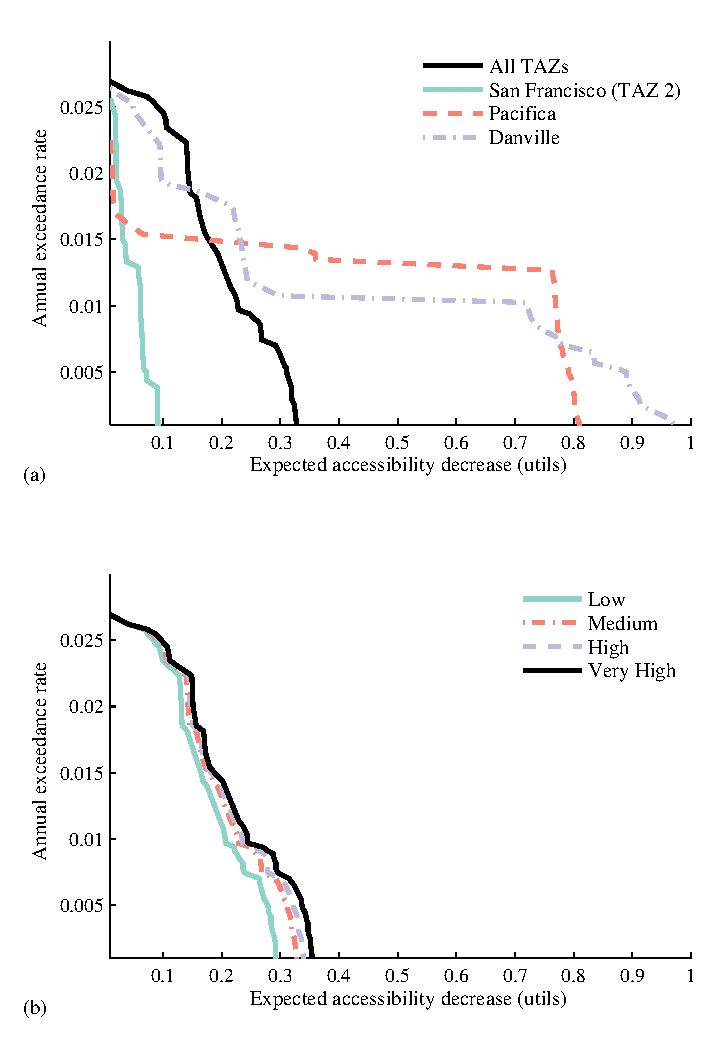
\includegraphics[width=4in]{FIGS/equity_acc_loss_curves.eps} 
\caption{Accessibility annual loss exceedance curve with a comparison by (a) case study TAZs and average over all TAZs and (b) income class; all curves are for medium income households with fewer cars than workers.}
\label{fig:acc_by_TAZ_and_income}
\end{figure}


\begin{table}
\caption{Income class definitions for the case study region, as defined by the local planning organization, the MTC~\cite{ory_personal_2013} and also translated to current 2014 USD using the consumer price index.}
\centering
\begin{tabular}{c|c|c}
\textbf{Income class}           & \textbf{Income range, 1989 USD} & \textbf{Income range, 2014 USD} \\
\hline
Low & $<$ \$25,000 & $<$ \$47,334\\
Medium &  \$25,000 - \$45,000 & \$47,334 - \$85,202\\
High & \$45,000 - \$75,000 & \$85,202 - \$142,004 \\
Very high & $>$ \$75,000 & $>$ \$142,004
\end{tabular}
\label{tab:incomes}
\end{table}


%These are classified by the income class and the relative number of vehicles (``cars'') to the number of household members that work as follows: a) low income, no cars, b) low income, workers $<$ cars, c) low income, workers $\geq$ cars, d) medium income, no cars, e) medium income, workers $<$ cars, cf) medium income, workers $\geq$ cars, g) high income, no cars, h) high income, workers $<$ cars, i) high income, workers $\geq$ cars, j) very high income, no cars, k) very high income, workers $<$ cars, and l) very high income, workers $\geq$ cars. Note, that very high income corresponds to households with a combined income of greater than \$142,004 USD (2014). Thus, for a given household, we can classify it into a socio-economic group by knowing the income class and the ratio of number of people working to the number of vehicles.

%We first assess the data availability for each of the segments. Each data point represents a trip by a person of a household, who is  modeled as an agent in the high-fidelity transportation model. The results suggest comparing households with at least one car, because for households without cars (no cars), only the low income class has reasonably many trips. 

%For the other income classes, the corresponding socio-economic groups of no car households is very small. 

%Thus, by themselves, the results from the other three socio-economic groups may not be fully representative of the true dynamics. However, the other nine socio-economic groups have a more reasonable representation. 


%\begin{figure}[h]
%\centering
%\includegraphics[width=6in]{FIGS/equity_dataset_count_bars.eps} 
%\caption{Percentage of total number of trips considered in the high-fidelity model by socio-economic group (determined by income class and household car ownership category) for the baseline (pre-earthquake) case.}
%\label{fig:car}
%\end{figure}




First, a higher ratio of cars to the number of people who work in a household corresponds to a higher expected decreases in accessibility (as seen by looking across a column in Figure~\ref{fig:acc_by_segment}).   
Households with more cars tend to take longer trips, and there is a relationship between needing to travel longer distances and needing an extra cars in a household. But there is only a weak trend between average trip length for a TAZ and the predicted impact on accessibility (Figure~\ref{fig:accLength}). Instead, we hypothesize that there are other latent variables correlated with both car ownership and accessibility risk (such as geographic location). In Section~\ref{sec:accDisc}, we will further explore the relationship between the percentage of car-based trips and accessibility risk.



%\begin{figure}[h!]
%\centering
%\includegraphics[width=4in]{FIGS/equity_trip_distance_income_cars_to_and_from_work.eps} 
%\caption{Distributions of commute trip length in 10-mile intervals  by a) income class segment, and b) car ownership segment,  (pre-earthquake)}
%\label{fig:lengthIncomeBars}
%\end{figure}

%\subsection{Impact of trip length}
%
\begin{figure}[htb!]
\centering
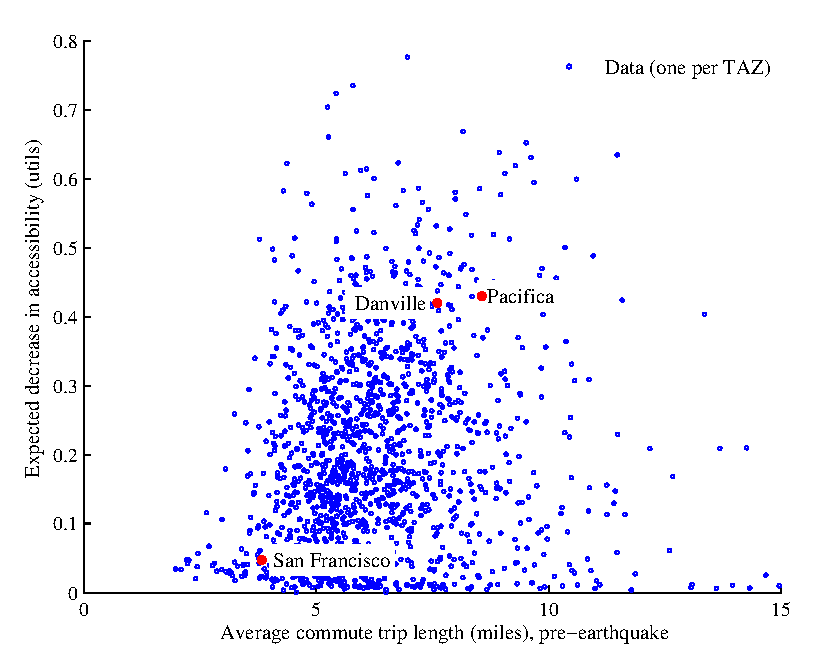
\includegraphics[width=4in]{FIGS/equity_accLengthv4.eps} 
\caption{Average pre-earthquake trip length versus change in expected accessibility for all TAZs in the study region. Each dot represents data from one TAZ, and red dots highlight the data points for the three case study communities.}
\label{fig:accLength}
\end{figure}



Second, controlling for car ownership, we see a fairly consistent distribution of risk across income classes.  For example, looking at households with fewer workers than cars (the middle column of Figure~\ref{fig:acc_by_segment}), the variation from TAZ to TAZ is much greater than the difference across income segments. Similarly, while trip lengths are slightly longer for higher income households, the differences are subtle. % (Figure~\ref{fig:lengthIncomeBars}{(a)}). 
Thus, for a given TAZ, the differences in impacts across incomes are not that great. There is, however, an unequal geographic distribution of wealth in the study region. Because of this, when we aggregate accessibility risk across TAZs, we see that accessibility risk rises slightly with increasing household income  (Figure~\ref{fig:acc_by_TAZ_and_income}{b}). 
%Therefore, even though the poor are generally the most vulnerable to natural disasters,  wealthier households in the San Francisco Bay area are more vulnerable than the other income groups to earthquake-related accessibility risk. [ Jack commented this out--I don't think this conclusion is fully justified. This assumes that greater reduction in accessibility utils is equivalent to greater "vulnerability" in general, but there are a few reasons why this isn't an apples-to-apples comparison.]


%we observe a gradual increase in expected accessibility losses down a column, such as down the right-hand column, representing households where the number of workers is greater than or equal to the number of cars (Figure~\ref{fig:acc_by_segment}{(c,f,i,l)}). However, this trend is more subtle than the trend with car ownership for a fixed income class.




Next, we consider TAZs indicated to have elevated risk.
%: due east of San Francisco, in the suburbs of San Jose, along the coastal and bay-side regions south of San Francisco (e.g., Millbrae and Pacifica), and in parts of San Francisco (south-central neighborhoods including the Westland Highlands and Glen Park neighborhoods). Geographic proximity to hazardous faults is one source of spatial variation. 
The San Francisco Peninsula is at risk of disruption from large magnitude San Andreas earthquakes, while the East Bay is at risk from slightly smaller but more frequent events on the Hayward Fault. Network simulations indicate that both Hayward and San Andreas earthquakes can cause accessibility problems for the East Bay. Figure~\ref{fig:scen_acc} shows realizations of a magnitude 6.85 Hayward event and a magnitude 7.45 San Andreas event---both show high accessibility losses in the East Bay.
%In contrast, the more moderate, more frequent Hayward event caused little impact for San Francisco; the San Andreas events were the chief contributors to the loss of accessibility in San Francisco. 
In contrast, the main predicted accessibility losses in San Francisco correspond primarily to San Andreas events.
Figures~\ref{fig:scen_acc}{c} and~\ref{fig:scen_acc}{d} provide one such example. Figures~\ref{fig:scen_acc}{e} and~\ref{fig:scen_acc}{f} show a lower magnitude event farther away from the main population centers: a magnitude 6.35 event in the Great Valley Pittsburg-Kirby Hills Fault. This shows how the more minor faults in the East Bay can contribute to that area's risk.
%, e.g., Figures~\ref{fig:scen_acc}{(d,f)}. 
%Note that in the three individual earthquake events shown---Hayward, M6.85, b) San Andreas, M7.45, c) San Andreas, M8.25---the accessibility losses are higher than average, since these are major events. 
The Figure~\ref{fig:scen_acc} results are for one specific socio-economic group, but comparable results for the other groups show the same patterns.


%\begin{figure}
%\centering
%\includegraphics[width=\textwidth]{../FIGS/equity_154_198_196.pdf} 
%\caption{Expected changes in accessibility for individual scenarios: a) Hayward, M7.05 (medium income, workers $<$ cars), b) San Andreas, M7.05 (medium income, workers $<$ cars), c) San Andreas, M8.25 (medium income, workers $<$ cars)}
%\label{fig:scen_acc}
%\end{figure}
\begin{figure*}[!htb]
    \centering
        \includegraphics[height=7in]{FIGS/accByEq.pdf}
    \caption{Bridge damage and corresponding accessibility losses by TAZ for medium income households with fewer cars than workers. The top three rows show results from specific events, while the bottom row has expected values calculated as a weighted average over all events.}
    % (the darker the color, the greater the losses). For expected bridge damage, the values are on a continuous scale from white to yellow to red in order of increasing annual likelihood of extensive or complete damage.}
\label{fig:scen_acc}
\end{figure*}


% loss exceedance curve
%Finally, we can examine the rates of loss exceedance. The annual rate, $\lambda$, of exceeding some threshold of network performance, as captured by change in accessibility, is estimated by summing the occurrence rates of all damage maps in which the performance measure exceeds the threshold: 
%\begin{equation}
%\lambda_{X \geq x} = \sum_{j'=1}^{J} w_{j'} \mathbbm{I}(X_{j'}\geq x)
%\label{eq:exceedance}
%\end{equation}
%where $x$ is an accessibility value threshold of interest and $X_{j'}$ is the accessibility value realization for the $j'^{th}$ damage map. The variable $w_{j'}$ is the occurrence rate of the $j'^{th}$ damage map.% ($w_j = \frac{w_j}{c}$ where $c$ is the number of damage map realizations per ground-motion intensity map). 
%%The function $\mathbbm{I}$ is an indicator function that evaluates to 1 if the argument, $x_j' \geq x$, is true and 0 otherwise. 
%The indicator function $\mathbbm{I}$  evaluates to 1 if the argument, $X_{j'} \geq x$, is true, and 0 otherwise.
%By evaluating $\lambda$ at different threshold values, we derive an exceedance curve, Figure~\ref{fig:acc_by_TAZ_and_income}). This graph shows a similar shape to the loss exceedance curves for other performance metrics for this case study network~\cite{miller_seismic_2014}. Note that the results are primarily valid in the 100 to 2475 year return periods, since this is the range chosen for the map selection optimization problem. As a sense of scale, if we use the average value over all TAZs for this 

Finally, we can examine the rates of loss exceedance (eq.~\ref{eq:exceedance}), as shown in Figure~\ref{fig:acc_by_TAZ_and_income}.  %Note these results are primarily valid in the 100 to 2475 year return periods, since this is the range chosen for the map selection optimization problem. %As a sense of scale, if we use the average value over all TAZs for this 
Recognizing that the impact varies significantly by TAZ, as indicated by Figure~\ref{fig:acc_by_segment},
%and the general lognormal shape of the accessibility cumulative distribution functions for a given event (Figure~\ref{fig:xxxx})
we also examine the accessibility loss exceedance curve for three communities: part of the San Francisco Financial District, Danville, and Pacifica. This part of the San Francisco Financial District  represents an area with relatively low expected changes in accessibility, whereas Danville and Pacifica are at an elevated risk in almost all socio-economic groups (Figure~\ref{fig:acc_by_segment}). 
The general trends are corroborated by the loss exceedance curves for these three communities (Figure~\ref{fig:acc_by_TAZ_and_income}{a} shows results for medium income households with fewer cars than workers). The average middle-class person from Danville in a household with fewer cars than workers is expected to experience travel-related losses up to 1 $util$ (or 75 minutes of extra travel time per day) after a rare earthquake. In contrast, a resident of San Francisco's Financial District has expected losses of only a tenth as much when considering the same exceedance rate. At annual rates of less than 0.01 (i.e., return periods greater than 100 years), Danville and Pacifica follow a similar general pattern that differs dramatically from that of San Francisco. 


%	\clearpage
	
	
	\subsection{Analysis for San Francisco Financial District}
	\label{sec:accSF}
	%So far we have focused on region-wide trends. However, we will now discuss the impacts at a local level for three communities, starting with one travel analysis zone (TAZ) of the downtown financial district of San Francisco (Figure~\ref{fig:equity_study_area}). As mentioned, San Francisco in general is expected to experience less loss in accessibility than most other communities. 
In this section, we will explore some possible explanations for why this San Francisco TAZ (Figure~\ref{fig:equity_study_area}) has lower expected accessibility losses than most other communities.
%something about walking!
First, the financial district of San Francisco differs dramatically from many other TAZs in that the percentage of trips made by car is relatively small (38\% versus an average of 85\% across all TAZs). Households traveling by foot or bike will be less influenced by network damage, because the model considers only damage to the road network and transit systems; thus, foot travel routes and travel times will not be affected in this model. We also observe that more trips by foot and bike correspond to destinations that are closer geographically. The impact of travel mode shift post-earthquake will be further explored in Section~\ref{sec:accDisc}.
 
 % loss exceedance curve. something about they take short trips.
 Second,  Figure~\ref{fig:time_distance_pdfs}{(a)} shows that the average time for a trip to and from work is about average for a TAZ in this region and also follows a similar distribution to that of the other TAZs. Figure~\ref{fig:time_distance_pdfs}{(b)} suggests a slight trend towards shorter trips, but the average trip distance for trips is only 7\% lower than the average for all trips region-wide. Since the trip time and length are relatively typical, but the accessibility is much lower than average, the trip time and length do not explain the differences in accessibility losses.
 
% may play a role in the relative accessibility risk for this TAZ, but other factors or combination of factors are likely more important. 

\begin{figure}
\centering
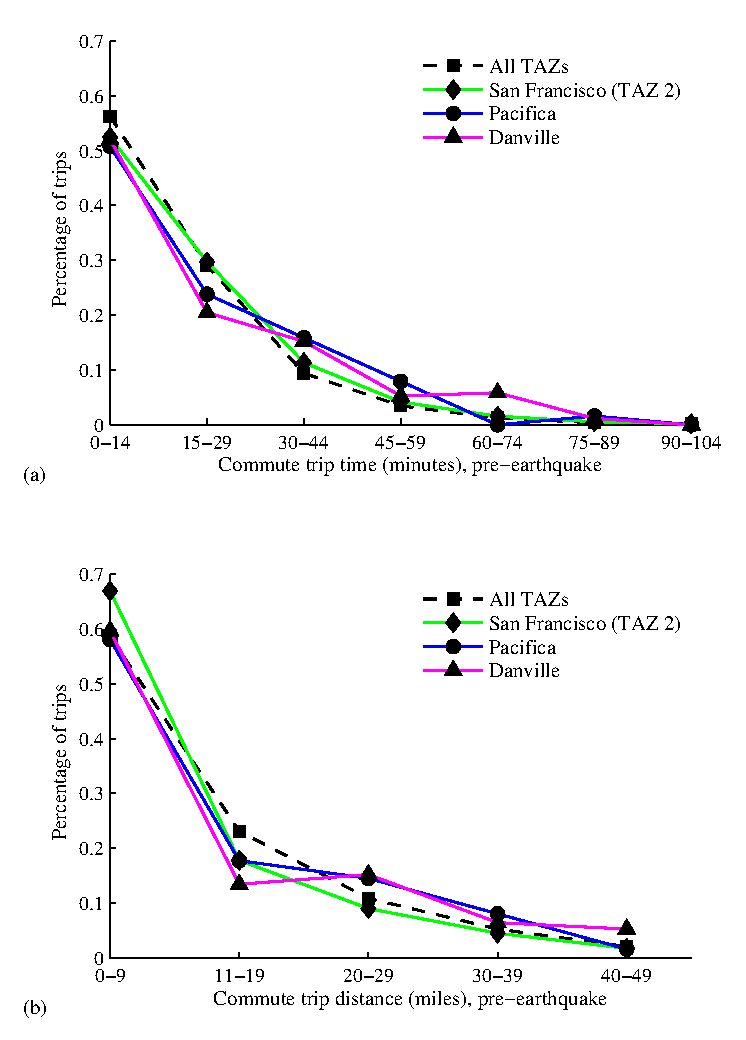
\includegraphics[width=4in]{FIGS/equity_trip_time_distance_pdfs_by_taz_to_work_and_from_work.eps} 
\caption{One-way commute trip information by (a) 15-minute time interval, and (b) 10-mile distance interval for 3 case study TAZs and the average over all TAZs.}
\label{fig:time_distance_pdfs}
\end{figure}



%\begin{figure}
%\centering
%\includegraphics[width=\textwidth]{../FIGS/equity_time_distance_SF.eps} 
%\caption{\textcolor{red}{TODO: add baseline, averaged over all TAZ?} Trip distributions for trips originating from San Francisco (TAZ 2)  after three earthquake events for a) trip length and b) trip time, as compared to the baseline.}
%\label{fig:time_distance_loss_sf}
%\end{figure}

%Third, as mentioned in the last section, areas away from the relatively more active Hayward and Calaveras faults in the East Bay have generally lower expected losses in accessibility. This is the case for this San Francisco TAZ. Specifically, the financial district is approximately 11 miles (18km) West of the closest segment of the Hayward Fault, with most areas even further away. Nonetheless, this is still close enough for some impact from these faults, e.g., as shown in Figure~\ref{fig:scen_acc}{(b)}. So, the results suggest that one factor to the relatively lower risk for San Francisco is being located on the San Francisco Peninsula (with a moderate separation distance from the East Bay faults), but not the key factor.
%%TODO: consider making a heat map of destinations from SF. Are they mostly avoiding East Bay bridges???

In summary, the data suggests that a major cause for the the low expected accessibility impact for the financial district of San Francisco is the lower relative dependence on cars for mobility. In the next section, we will contrast the San Francisco example with results from Pacifica, another Peninsula community that, nonetheless, is expected to be at high risk of losses in accessibility.
%	\clearpage
	
	
	\subsection{Analysis for Pacifica}
	\label{sec:accPacifica}
	%In this section, we will explore the causes of the high risk of losses in accessibility for Pacifica, CA.
%Like Danville, Pacifica is at high risk of losses in accessibility, but for different reasons.
%While trip length and bridge vulnerability play a big role in the accessibility risk for Danville, physical conditions contribute significantly to the risk of Pacifica, CA (Figure~\ref{fig:equity_study_area}). \textcolor{red}{TODO: write section}
%In contrast to downtown San Francisco, Pacifica, CA  (Figure~\ref{fig:equity_study_area}) has a high risk of losses in accessibility. We will now explore why. 

%Based on seismic hazard (e.g., Figures~\ref{fig:haz475} and \ref{fig:haz2475}), we might not suspect that Pacifica, CA would be at an elevated risk of accessibility losses across most market segments. In addition, the percentage of pre-earthquake car-based trips is around average for the case study area (88\% versus an average of 85\%). 
%In contrast to most other regions, however, Pacifica is wedged between the Pacific Ocean to the West and the coastal mountains to the East. Indeed, the main access road is California Highway 1, which has various vulnerable bridges included in the case study dataset. There are no viable alternative routes on local roads. Since almost all trips are by car from Pacifica and the average trip length is much longer than the region-wide average (108\% longer), the road issue is particularly serious.

We might not suspect that Pacifica, CA would be at an extremely elevated risk of accessibility losses across most market segments, as compared to other communities, because it is not unusually close to a major earthquake fault. In addition, the percentage of pre-earthquake car-based trips is around average for the case study area (88\% versus an average of 85\%). 
In contrast to most other regions, however, Pacifica is wedged between the Pacific Ocean to the West and the coastal mountains to the East. Indeed, the main access road is California Highway 1, which has various vulnerable bridges included in the case study dataset. There are no viable alternative routes on local roads. Since almost all trips are by car from Pacifica and the average trip length is much longer than the region-wide average (108\% longer), the road issue is particularly serious.

As a comparison, consider the next main town along the Pacific coast, Half Moon Bay, about 13 miles South. Half Moon Bay has significantly lower expected accessibility losses compared to Pacifica, as illustrated in Figure~\ref{fig:scen_acc} with cities labeled for reference in Figure~\ref{fig:pac}. 
This corresponds to an expected accessibly loss of 0.43 $utils$ per day for a person in Pacifica in middle income household with fewer cars than workers, given an event in the dataset. In comparison, a similar person in Half Moon Bay is expected only a 0.11 $utils$ loss.
%Yo! Mahalia HMB straddles TAZs 295 and 296. Pacifica is 224.
% For example, for the socio-economic group with middle income households with fewer cars than people who work (Figure~\ref:{fig:scen_acc}{(e)}, the expected accessibility decrease is estimated at xxx $utils$ for Pacifica and only xxx $utils$ for Half Moon Bay. 
While the seismic hazard is similar, the population is about one third the size, so there is less demand for the limited road capacity~\cite{u.s._bureau_of_the_census_united_2010}. Furthermore, and likely most significantly, Half Moon Bay has a key alternative to California Highway 1, California Highway 92, which links to Silicon Valley and the main highways of that region (US-101 and I-280). The differences in the road topology are illustrated in Figure~\ref{fig:pac}. Since Pacifica, CA is unusually reliant on one road with key vulnerabilities for access, it has an elevated risk for losses in accessibility.

%In addition, we see that under normal pre-earthquake conditions, people in Pacifica take much longer trips on average, around 8.57 miles on average, vs. a region-wide average of 6.35 mies

%\begin{figure}
%\centering
%\includegraphics[width=6in]{../FIGS/equity_time_distance_Pacifica.eps} 
%\caption{\textcolor{red}{TODO: add baseline} Trip distributions for trips originating from Pacifica (TAZ 224)  after three earthquake events for a) trip length and b) trip time, as compared to the baseline.}
%\label{fig:time_distance_loss_danville}
%\end{figure}


\begin{figure*}[t]
    \centering
    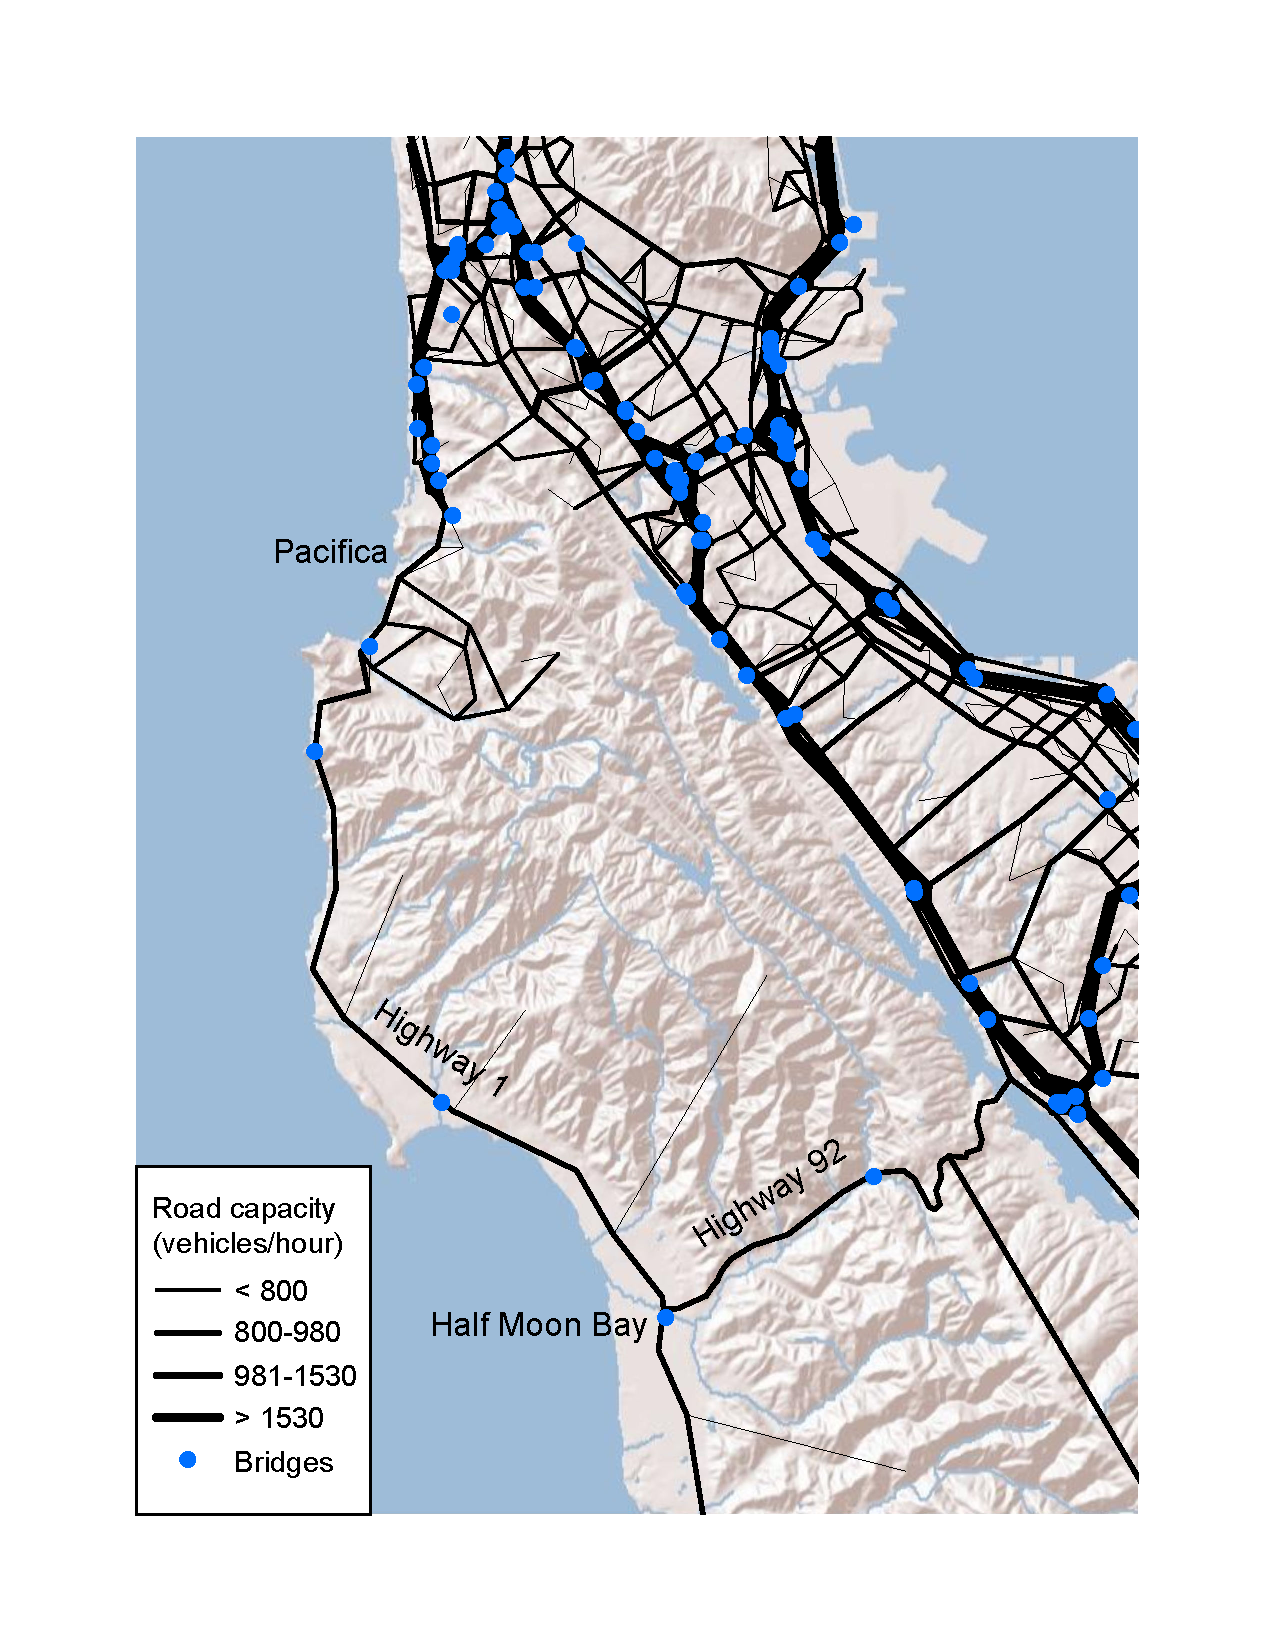
\includegraphics[height=7in]{FIGS/equity_hmb.pdf} 
\caption{Differences in road access: limited roads in and out of Pacifica, CA, but an extra access highway for Half Moon Bay, CA.}
\label{fig:pac}
\end{figure*}


%	\clearpage
	
	
	\subsection{Analysis for Danville}
	\label{sec:accDanville}
	%While physical conditions contribute significantly to the risk of Pacifica, CA, trip length and bridge vulnerability play a big role in the accessibility risk for Danville, CA (Figure~\ref{fig:equity_study_area}). 

We will first examine the trip length characteristics for Danville. %As illustrated in Figure~\ref{fig:time_distance_pdfs}, t
The distribution of pre-earthquake commute trips from Danville is shifted towards both longer distance and longer time than the communities we have studied so far; for example, the average length of a trip from Danville is 85\% longer than the average over all trips originating from any TAZ. More specifically, there is a relatively higher proportion of trips taking 60-74 minutes and traveling over 40 miles than in the other communities. The consequence of these longer trips is more opportunities to be impacted by a road closure, simply because more roads and bridges will be used. Moreover, the road layout near Danville mandates many highway trips, which increase the likelihood of crossing bridges; bridges are the part of the network for which we model the vulnerability. 

%\begin{figure}
%\centering
%\includegraphics[width=\textwidth]{../FIGS/equity_time_distance_Danville.eps} 
%\caption{Trip distributions for trips originating from Danville (TAZ 1161) for change over baseline after three earthquake events for a) trip length and b) trip time.}
%\label{fig:time_distance_loss_danville}
%\end{figure}

Next, we look at patterns of expected bridge damage. Bridge damage is important for many regions, including Danville, because the percentage of car-based trips is high (85\% of all trips on average, and also 85\% of Danville-origin trips). For damage map realizations for the three  earthquake events we introduced---M6.85 Hayward Fault, M7.45 San Andreas Fault, M6.35 Great Valley Fault---some bridges in the Oakland area are in the extensive or greater damage state (Figure~\ref{fig:scen_acc}{(a,c,e)}). These correspond to bridge closures in the model. In addition, in the first two cases, there are closures to the north of Danville, which represents one of the two main travel routes from Danville. There are also scattered closed bridges to the west of Danville, a top travel corridor for people of Danville because of the workplace centers in San Francisco, Oakland, and Silicon Valley (all to the west). As for transit, in the first two events, all BART lines are closed, so there are limited alternatives to the popular road routes. The result is that the residents of Danville have reduced access to their normal destinations after all these events. 

We can also look at bridge damage in a probabilistic event-set-based manner. The expected damage over all events represents the annual rate of a bridge being in the extensive or complete damage state for an extensively-sampled, hazard-consistent set of damage maps (Figure~\ref{fig:scen_acc}{(g)}). This figure indicates that bridges in the Oakland-Berkeley area are particularly likely to be damaged. We also see a few high likelihood bridges to the North of Danville. Thus, the data suggests that the relative position of high-risk bridges to Danville contributes to this community's accessibility risk.

%\begin{figure*}[t]
%    \centering
%    \begin{tabular}{cc}
%    \includegraphics[width=0.4\textwidth]{../FIGS/bridge_scen_154.eps} &
%    \includegraphics[width=0.4\textwidth]{../FIGS/bridge_scen_198.eps} \\
%     (a) Hayward, M7.05 & (b) San Andreas, M7.05 \\ 
%    \includegraphics[width=0.4\textwidth]{../FIGS/bridge_scen_196.eps} &
%        \includegraphics[width=0.4\textwidth]{../FIGS/equity_probDamageBig.eps} \\
%        (c) San Andreas, M8.25 & (d) Weighted average   
%    \end{tabular}
%\caption{Bridge damage state: a) after M7.05 Hayward, b) after M7.05 San Andreas, c) after M8.25 San Andreas, d) expected damage over all events (red is high likelihood  of extensive or complete bridge damage, and white is low likelihood).}
%\label{fig:bridge_ds}
%\end{figure*}



%	\clearpage

	\subsection{Impact of travel mode shifts and regional variations in travel mode patterns}
	\label{sec:accDisc}
	%In this section, we will discuss generalizable trends of factors contributing to a community's accessibility risk, which offer insight into possible opportunities for risk mitigation. 
%
%\subsection{Trends by car ownership class}
%\label{sec:carEquity}
%From Section~\ref{sec:accAll}, we notice that the ratio of cars to the number of people who work in a household is strongly correlated with accessibility risk; a higher ratio corresponds to higher expected decreases in accessibility. This result could stem from a few causes. 
%
%First, we have seen that households living in communities, such as Danville, CA, that on average take longer trips, are at greater risk. Thus, we might expect households at greater risk, i.e., households with more cars, to take longer trips. This is indeed the case (Figure~\ref{fig:lengthIncomeBars}{(b)}). However, as suggested in Section~\ref{sec:accSF}, trip length is not fully predictive. In fact, there is only a weak trend between average trip length for a TAZ before any earthquake and the predicted impact on accessibility (Figure~\ref{fig:accLength}).
%
%Instead, we predict that there are other latent variables correlated with car ownership. For example, the geographic distribution of people without cars varies. Additionally, in Section~\ref{sec:acctravelshift}, we will further explore the correlation between the percentage of car-based trips and accessibility risk. We will show that TAZs with fewer car-based trips, tend to have lower risk of accessibility losses.
%
%
%\begin{figure}
%\centering
%\includegraphics[width=5in]{../FIGS/equity_trip_distance_income_cars_to_and_from_work.eps} 
%\caption{Distributions of commute trip length in 10-mile intervals  by a) income class segment, and b) car ownership segment,  (pre-earthquake)}
%\label{fig:lengthIncomeBars}
%\end{figure}
%
%%\subsection{Impact of trip length}
%%
%\begin{figure}
%\centering
%\includegraphics[width=6in]{../FIGS/equity_accLength.eps} 
%\caption{Trip length (pre-earthquake) versus change in total accessibility per person per day}
%\label{fig:accLength}
%\end{figure}
%
%
%
%
%\subsection{Trends by income class}
%Controlling for car ownership, we see a fairly equitable distribution of risk across income class segments.  For example, by looking at households with fewer workers than cars, the variation from TAZ to TAZ is significantly more striking than the difference across income segments (Figure~\ref{fig:acc_by_segment}{(b,e,h,k)}). Similarly, while trip lengths are slightly longer for higher income households, the differences are subtle (Figure~\ref{fig:lengthIncomeBars}{(a)}).
%
%
%Thus, for a given TAZ, the differences across incomes are not that great. However, there is an unequal geographic distribution of wealth in the San Francisco Bay Area. Because of this, when we aggregate accessibility risk across TAZs, we see that accessibility risk rises with increasing household income  (Figure~\ref{fig:acc_by_TAZ_and_income}{(b)}). Therefore, even though the poor are generally the most vulnerable to climatological and geophysical hazards and disasters, such as hurricanes, floods and earthquakes~\cite{fothergill_race_1999},  wealthier households in the San Francisco Bay area are more vulnerable than the other income groups to earthquake-related accessibility risk.
%
%%\begin{figure}
%%\centering
%%\includegraphics[width=6in]{../FIGS/equity_accCCDF_by_Income.eps} 
%%\caption{Trip length (pre-earthquake) versus change in total accessibility (households with the number of cars less than the number of workers) }
%%\label{fig:equity_accCCDF_by_Income}
%%\end{figure}
%
%
%
%%look above for subfigure b that has length vs. income segment
%
%%but note that income is tied to car ownership...
%
%
%
%
%
%%\begin{figure}
%%\centering
%%\includegraphics[width=\textwidth]{../FIGS/equity_dataset_count_matrix_hh.eps} 
%%\caption{Household-by-household distribution of car ownership by income class (as percentage of total number of households)}
%%\label{fig:car}
%%\end{figure}
%\begin{figure}[h]
%\centering
%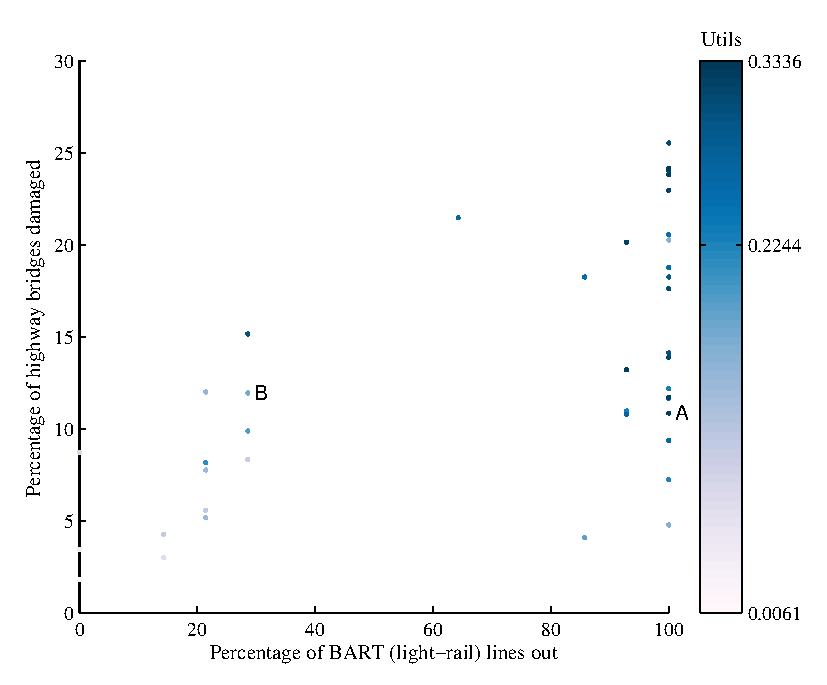
\includegraphics[width=6in]{../FIGS/equity_bart_bridges_acc.eps} 
%\caption{Percentage of BART (heavy-rail) lines not operational versus percentage of highway bridges damaged for each of the 40 events. The values are color-coded by the average loss in accessibility per day per person over all TAZs (for the market segment of households with the number of cars less than the number of workers). Two events discussed in this section are marked by the letters A and B.}
%\label{fig:bartBri}
%\end{figure}
%
%\subsection{Impact of travel mode shifts and regional variations in travel mode patterns on accessibility risk} \label{sec:acctravelshift}

%\subsection{Impact to accessibility risk of both travel mode shifts and regional variations in travel mode patterns} \label{sec:acctravelshift}
%Two key factors related to the resilience of a community to transportation network damage are the post-earthquake functionality of the relevant transit systems, and  how conducive a community is for trips by bike or by foot. 

%In this section, we will compare patterns of transit system damage with patterns of travel mode shifts after earthquake events, and then discuss the corresponding trends in accessibility impact. Then, we will examine the correlation between a community's walkability and bike friendliness, as measured by the percentage of total trips made by those travel modes, and the expected losses in accessibility by community. 





\begin{figure}[H]
\centering
\includegraphics[width=5in]{FIGS/equity_bart_bridges_acc3.eps} 
\caption{Percentage of BART (heavy-rail) lines not operational versus percentage of highway bridges damaged, where each data point corresponds to one earthquake damage map. The values are color-coded by the average loss in accessibility per day per person over all TAZs for households with the fewer cars than people who work. Two events discussed in this section are marked by the letters A and B.}
\label{fig:bartBri}
\end{figure}



First, we compare patterns of transit system damage with patterns of travel mode shifts after earthquake events. Over all the simulated events, taking a weighted average by the annual likelihood of each event, we see a reduction in transit ridership (25\% weighted average decrease from the base case). This is not surprising. The heavy rail systems (BART and Caltrain) are not fully operational in most of the forty simulated events (Table~\ref{tab:transit}), and these have heavy ridership. The light rail systems (VTA and Muni light rail) also suffered losses in many events (Table~\ref{tab:transit}). %As detailed in~\cite{miller_seismic_2014}, with regards to the other transit systems, trans-bay and cross-county bus lines were suspended in the forty events and the baseline case; main local buses are modeled as operational, although with possible delays; and ferries are modeled as operational.
% in only 13 out of the 40 earthquake events, are more than 50\% of the BART lines running, with similar trends for other transit systems. 
 The result is an average increase in the percentage of trips by the other modes (foot, car, and bike). 

\begin{table*}
\centering
\begin{tabular}{c||c|c|c|c}
\textbf{Functionality}           & \textbf{BART} & \textbf{Caltrain} & \textbf{Muni Light Rail} & \textbf{VTA Light Rail}  \\
\hline
Full & 3 & 13 & 25 & 9\\
50-99\%  & 10 & 0 & 15 & 0\\
1-49\%  & 8 & 0 & 0 & 0\\
None & 19 & 27 & 0 & 31\\
\end{tabular}
\caption{Transit network functionality as a count out of the forty simulated events for BART, Caltrain, Muni Light Rail, and VTA Light Rail. Functionality is measured by the percentage of lines that are operational given a damage map (based on a ground-motion intensity map). }
\label{tab:transit}
\end{table*}


%The result is approximately a 1.3????\% change in travel mode. This is roughly consistent with the 14\% change in travel mode estimated after the 1994 Northridge earthquake~\cite{gordon_transport-related_1998}.

A notable exception is the M6.35 Great Valley, Pittsburg-Kirby Hills Fault earthquake event, as illustrated in Figure~\ref{fig:scen_acc}{(e,f)}. In this event, there were no line closures on the major transit systems (BART, Caltrain, Muni, and VTA Light Rail). There were, however, some bridge closures on the highways (Figure~\ref{fig:scen_acc}{(e)}). The result was a slight increase in transit ridership and also in trips by foot.

In general, accessibility impact grows with increasing number of damaged transit lines, particularly in combination with high numbers of damaged bridges (Figure~\ref{fig:bartBri}). The results do not conclusively show that transit is a key contributor to accessibility risk, but based on individual examples, the data suggests this conclusion. For example, in the set of forty events analyzed with the high-fidelity model, the M6.85 Hayward Rogers-Creek and the M7.45 Northern San Andreas Fault event both have a similar number of damaged bridges (around 11\%); these are noted by points A and B respectively in Figure~\ref{fig:bartBri}. These correspond to the bridge damage and accessibility maps in Figures~\ref{fig:scen_acc}{(a,b)} and \ref{fig:scen_acc}{(c,d)} respectively.  However, this Hayward Rogers-Creek event has significantly higher accessibility impact. Similarly, the transit impact was different. This Northern San Andreas event had only 4 of the 14 BART lines, all Caltrain, and all VTA Light Rail lines not operational, whereas this Hayward Rogers-Creek event had all 14 of the 14 BART lines, all Caltrain, all VTA Light Rail and 3 of the 8 Muni light rail lines not operational.  Thus, the Hayward Rodgers-Creek event featured significantly higher losses to the transit network.
%Thus, the transit lines were impacted significantly differently. 
Moreover, the differences in accessibility results could not have been predicted from simpler models focusing on bridge portfolio losses, because the percent of damaged bridges was about the same, and the San Andreas event actually corresponded to a greater increase in fixed-demand travel time.

%In general, accessibility impact grows with increasing number of damaged transit lines, particularly in combination with high numbers of damaged bridges (Figure~\ref{fig:bartBri}). The results do not conclusively show that transit is a key contributor to accessibility risk, but based on individual examples, the data suggests this conclusion. For example, the  M7.05 Hayward Rogers-Creek Fault event discussed above and the M7.45 Northern San Andreas Fault event both have a similar number of damaged bridges; these are noted by points A and B respectively in Figure~\ref{fig:bartBri}. However, this Hayward Rogers-Creek event has significantly higher accessibility impact. Similarly, the transit impact was different. This Northern San Andreas event had only 4 of the 14 BART lines, all Caltrain and all VTA Light Rail lines not operational, whereas this Hayward Rogers-Creek event had all 14 of the 14 BART lines, all Caltrain, all VTA Light Rail and 3 of the 8 Muni light rail lines not operational. Thus, the transit lines were significantly differently impacted. Furthermore, the accessibility results could not have been predicted from the efficient transportation model introduced in  Section~\ref{sec:caseMet}.

% For example, the xxxx event and the xxxx event have similar number of damaged bridges and a similar travel time predicted from the efficient fixed-demand model. However, the xxxx event has significantly higher accessibility impact. Similarly, the transit impact was different. The xxxx event had xxx and the xxxx event had xxxx.

Second, we examine the correlation between a community's walkability, as measured by the percentage of total trips made by that travel mode, and the expected decrease in accessibility by community. We see that an increased percentage of pre-earthquake trips on foot corresponds to a lower average decrease in accessibility (Figure~\ref{fig:walkingVsAcc}). This result corroborates the specific example of the San Francisco Financial District we saw in Section~\ref{sec:accSF}. Furthermore,  on average, the number of by-foot trips slightly increases after the earthquake events where road congestion worsens. This model result is consistent with the observations after the 1995 Kobe earthquake, in which many commuters switched to walking and biking (``non-mechanized modes'') in the weeks after the earthquake~\cite{gordon_transport-related_1998}. In conclusion, the data suggests that TAZs, i.e. communities, which have a greater walkability are also more resilient to earthquake-related accessibility risk. 

\begin{figure}[H]
\centering
\includegraphics[width=5in]{FIGS/equity_footVsAccv3.eps} 
\caption{Percentage of total trips by foot (pre-earthquake) versus decrease in total accessibility, measured in $utils$ per day (for households with the number of cars less than the number of workers). Each dot represents data from one TAZ, and red dots highlight the data points for the three case study communities: San Francisco financial district, Danville, and Pacifica.}
\label{fig:walkingVsAcc}
\end{figure}


%\subsection{Limitations}
%	\clearpage

\section{Conclusions}
\label{sec:accConc}
We have shown how mode-destination accessibility can be used to link post-earthquake infrastructure damage to the impact on human welfare and enables identifying at-risk geographic and demographic groups in a region. 
%Here we have shown a framework for coupling mode-destination accessibility with a quantitative seismic-risk assessment to identify at-risk populations and measure the accompanying impacts on human welfare.
Adopting this state-of-the-art performance metric from the urban planning community, we have illustrated its use for seismic risk assessment and mitigation through a case study of the San Francisco Bay Area. For the case study, we considered a set of 40 hazard-consistent earthquake scenarios, ground-motion intensity maps, damage maps, and corresponding annual rates of occurrence. For each damage map, we performed a detailed activity-based travel model calculation that includes the road network, transit networks, walking and biking options, variable travel demand, and mode choice. We used this data and model to compute the mode-destination accessibility, a performance measure for each community and each socio-economic group (defined by income class and car ownership). 


%, we analyzed impact with a high-fidelity, activity-based travel model that includes the road network, transit networks, walking and biking options, variable travel demand, and mode choice. 
%
%Furthermore, we have proposed a model that captures transport mode choice and the interdependencies of the roads and transit systems. We have nested this network performance model within an event-based probabilistic seismic risk framework. 
%%example
%Using a set of 40 hazard-consistent earthquake scenarios, ground-motion intensity maps, and damage maps, we analyzed impact with a high-fidelity, activity-based travel model that includes the road network, transit networks, walking and biking options, variable travel demand, and mode choice. 
%%In the case study, we first simulated a large set of earthquake scenarios, ground-motion intensity maps, and damage maps. Then, we used optimization to select a subset of the maps. After that, for each of the selected maps, we processed the data for analysis in a high-fidelity, activity-based travel model that includes the road network, transit networks, walking and biking options, variable travel demand, and mode choice. 
%%First, we simulated earthquake scenarios. Adding on spatial correlation, we then simulated ground-motion intensity maps. From these, we generated structural-component and network-component damage maps. We then computed basic network performance (travel time delay) with an efficient travel model. Using an optimization procedure, we selected a subset of these maps for modeling in a high-fidelity transportation model used by the local transportation authorities. The key differences, however, are a) we simulated earthquake damage to bridges, roads, and transit lines, and b) we automated the procedure to run many events in an event-based probabilistic risk framework. 
%We used this data and model to compute the mode-destination accessibility, a state-of-the-art performance measure for each community and each socio-economic group (defined by income class and car ownership). 

%WIthin this broader context, we focus on three communities whose experiences after future earthquakes are expected to differ considerably.

%although we saw this,
We saw stark differences in accessibility from location to location. The far East Bay, south San Jose and some communities south of San Francisco were particularly at risk. We found that these geographic trends persisted across income classes and car ownership groups. Nonetheless higher income households with more cars than workers had higher average accessibility losses than other socio-economic groups. One key reason is the geographic clustering of these households in higher-risk areas. Another factor is that these households tend to take longer daily trips, thus crossing more roads and bridges and possibly increasing the likelihood of disruption.

%despite these differences, ...
This study also demonstrated that travel modes shift after an earthquake, and communities that can more easily adjust are predicted to experience lower post-earthquake losses in accessibility. The results suggest that the walkability of a community, as measured by the percentage of pre-earthquake trips by foot, is closely linked to reduced accessibility risk. 
%We also found that one adaptation measure after major earthquakes is an increased likelihood to walk or bike. 
We also found that in almost all of the simulated earthquake events, the transit system is predicted by this model to be severely impacted. The result is a reduced mode share for transit and increased trips by the other modes (car, walking, and bike). Thus, this study suggests that not modeling transit disruption can lead to a nonconservative estimate of seismic risk of transportation systems. The model shows, however, that when transit is not damaged---which is very rare for this case study---ridership increases.

%in conclusion, xxx has yy important applications:
In conclusion,  mode-destination accessibility offers important insights into the relationship between damage to physical infrastructure and impacts on human welfare. 
Using a detailed transportation network model, computationally efficient analysis strategies, and this refined measures of impact, we obtain new insights about users' risk, and obtain metrics that are usable by urban planners responsible for long-term management of  transportation systems.
This approach provides a foundation for future work in risk mitigation and policy to reduce the vulnerability of at-risk communities. It  suggests that initiatives making communities more conducive for cycling and walking to work can increase resiliency to disasters. It also provides a method to quantify societal benefits of upgrading various aspects of a regions' transportation systems.

%increasing bike friendliness and walkability can increase resiliency.

\section{Acknowledgements}
\label{sec:accAckn}
We thank Dave Ory at the Metropolitan Transportation Commission (MTC) and Tom Shantz and Loren Turner at Caltrans for motivating discussions and providing the case study data. The first author thanks the support of the NSF and Stanford Graduate Research Fellowships. This work was supported in part by the National Science Foundation under NSF grant number CMMI 0952402. Any opinions, findings and conclusions or recommendations expressed in this material are those of the authors and do not necessarily reflect the views of the National Science Foundation.


%% The Appendices part is started with the command \appendix;
%% appendix sections are then done as normal sections
%% \appendix

%% \section{}
%% \label{}

%% References
%%
%% Following citation commands can be used in the body text:
%% Usage of \cite is as follows:
%%   \cite{key}         ==>>  [#]
%%   \cite[chap. 2]{key} ==>> [#, chap. 2]
%%

%% References with BibTeX database:

\bibliographystyle{elsarticle-num}
\bibliography{newfile}%subset_journal} %change via grep -v "url =" file.bib > newfile.bib %http://tex.stackexchange.com/questions/26318/disabling-urls-in-bibliography


%% Authors are advised to use a BibTeX database file for their reference list.
%% The provided style file elsarticle-num.bst formats references in the required Procedia style

%% For references without a BibTeX database:

% \begin{thebibliography}{00}

%% \bibitem must have the following form:
%%   \bibitem{key}...
%%

% \bibitem{}

% \end{thebibliography}

\end{document}